\documentclass{book}
\usepackage[a4paper,top=2.5cm,bottom=2.5cm,left=2.5cm,right=2.5cm]{geometry}
\usepackage{makeidx}
\usepackage{natbib}
\usepackage{graphicx}
\usepackage{multicol}
\usepackage{float}
\usepackage{listings}
\usepackage{color}
\usepackage{ifthen}
\usepackage[table]{xcolor}
\usepackage{textcomp}
\usepackage{alltt}
\usepackage{ifpdf}
\ifpdf
\usepackage[pdftex,
            pagebackref=true,
            colorlinks=true,
            linkcolor=blue,
            unicode
           ]{hyperref}
\else
\usepackage[ps2pdf,
            pagebackref=true,
            colorlinks=true,
            linkcolor=blue,
            unicode
           ]{hyperref}
\usepackage{pspicture}
\fi
\usepackage[utf8]{inputenc}
\usepackage{mathptmx}
\usepackage[scaled=.90]{helvet}
\usepackage{courier}
\usepackage{sectsty}
\usepackage{amssymb}
\usepackage[titles]{tocloft}
\usepackage{doxygen}
\lstset{language=C++,inputencoding=utf8,basicstyle=\footnotesize,breaklines=true,breakatwhitespace=true,tabsize=4,numbers=left }
\makeindex
\setcounter{tocdepth}{3}
\renewcommand{\footrulewidth}{0.4pt}
\renewcommand{\familydefault}{\sfdefault}
\hfuzz=15pt
\setlength{\emergencystretch}{15pt}
\hbadness=750
\tolerance=750
\begin{document}
\hypersetup{pageanchor=false,citecolor=blue}
\begin{titlepage}
\vspace*{7cm}
\begin{center}
{\Large My Project }\\
\vspace*{1cm}
{\large Generated by Doxygen 1.8.3.1}\\
\vspace*{0.5cm}
{\small Sun Jan 25 2015 23:20:17}\\
\end{center}
\end{titlepage}
\clearemptydoublepage
\pagenumbering{roman}
\tableofcontents
\clearemptydoublepage
\pagenumbering{arabic}
\hypersetup{pageanchor=true,citecolor=blue}
\chapter{Module Index}
\section{Modules}
Here is a list of all modules\-:\begin{DoxyCompactList}
\item \contentsline{section}{Constants}{\pageref{group___d_e_f_i_n_e}}{}
\item \contentsline{section}{Typedefs/\-Enums}{\pageref{group___t_y_p_e_d_e_f_s}}{}
\item \contentsline{section}{G\-L\-U\-I variables}{\pageref{group___g_l_u_i___v_a_r_i_a_b_l_e_s}}{}
\end{DoxyCompactList}

\chapter{Hierarchical Index}
\section{Class Hierarchy}
This inheritance list is sorted roughly, but not completely, alphabetically\+:\begin{DoxyCompactList}
\item \contentsline{section}{Block}{\pageref{class_block}}{}
\item \contentsline{section}{Bullet\+Manager}{\pageref{class_bullet_manager}}{}
\item \contentsline{section}{Collision}{\pageref{class_collision}}{}
\item \contentsline{section}{Connection}{\pageref{class_connection}}{}
\begin{DoxyCompactList}
\item \contentsline{section}{My\+Connection}{\pageref{class_my_connection}}{}
\end{DoxyCompactList}
\item \contentsline{section}{Creep\+Manager}{\pageref{class_creep_manager}}{}
\item Drawable\begin{DoxyCompactList}
\item \contentsline{section}{Button}{\pageref{class_button}}{}
\item \contentsline{section}{Drawable\+Container}{\pageref{class_drawable_container}}{}
\end{DoxyCompactList}
\item \contentsline{section}{Game}{\pageref{class_game}}{}
\item \contentsline{section}{Game\+Object}{\pageref{class_game_object}}{}
\begin{DoxyCompactList}
\item \contentsline{section}{Bullet}{\pageref{class_bullet}}{}
\item \contentsline{section}{Creep}{\pageref{class_creep}}{}
\item \contentsline{section}{Hero}{\pageref{class_hero}}{}
\item \contentsline{section}{Tower}{\pageref{class_tower}}{}
\end{DoxyCompactList}
\item \contentsline{section}{Game\+State}{\pageref{class_game_state}}{}
\begin{DoxyCompactList}
\item \contentsline{section}{Game\+Over\+State}{\pageref{class_game_over_state}}{}
\item \contentsline{section}{Main\+Game\+State}{\pageref{class_main_game_state}}{}
\item \contentsline{section}{Main\+Menu\+State}{\pageref{class_main_menu_state}}{}
\end{DoxyCompactList}
\item \contentsline{section}{Path}{\pageref{class_path}}{}
\item \contentsline{section}{Player}{\pageref{class_player}}{}
\item \contentsline{section}{Sound\+Manager}{\pageref{class_sound_manager}}{}
\item \contentsline{section}{State\+Manager}{\pageref{class_state_manager}}{}
\item \contentsline{section}{Team}{\pageref{class_team}}{}
\item \contentsline{section}{Tower\+Manager}{\pageref{class_tower_manager}}{}
\item \contentsline{section}{Window}{\pageref{class_window}}{}
\end{DoxyCompactList}

\chapter{Class Index}
\section{Class List}
Here are the classes, structs, unions and interfaces with brief descriptions\-:\begin{DoxyCompactList}
\item\contentsline{section}{\hyperlink{class_ball}{Ball} \\*Simple class for defining ball objects }{\pageref{class_ball}}{}
\item\contentsline{section}{\hyperlink{class_image}{Image} \\*Represents a B\-M\-P image }{\pageref{class_image}}{}
\item\contentsline{section}{\hyperlink{struct_my_color}{My\-Color} \\*To store the color attribute in R\-G\-B format }{\pageref{struct_my_color}}{}
\item\contentsline{section}{\hyperlink{struct_my_struct}{My\-Struct} \\*To store three dimensional variables like position, velocity, etc }{\pageref{struct_my_struct}}{}
\item\contentsline{section}{\hyperlink{class_my_thread}{My\-Thread} \\*Extends the functionality of Class \hyperlink{class_thread}{Thread} }{\pageref{class_my_thread}}{}
\item\contentsline{section}{\hyperlink{class_particle}{Particle} \\*Snow particles in background }{\pageref{class_particle}}{}
\item\contentsline{section}{\hyperlink{class_theme}{Theme} \\*To store features of theme }{\pageref{class_theme}}{}
\item\contentsline{section}{\hyperlink{class_thread}{Thread} \\*Class to be inherited by \hyperlink{class_my_thread}{My\-Thread} }{\pageref{class_thread}}{}
\item\contentsline{section}{\hyperlink{class_wall}{Wall} \\*\hyperlink{class_wall}{Wall} object to define boundaries of window/box }{\pageref{class_wall}}{}
\end{DoxyCompactList}

\chapter{File Index}
\section{File List}
Here is a list of all documented files with brief descriptions\+:\begin{DoxyCompactList}
\item\contentsline{section}{inc/{\bfseries Block.\+hpp} }{\pageref{_block_8hpp}}{}
\item\contentsline{section}{inc/{\bfseries Bullet.\+hpp} }{\pageref{_bullet_8hpp}}{}
\item\contentsline{section}{inc/{\bfseries Bullet\+Manager.\+hpp} }{\pageref{_bullet_manager_8hpp}}{}
\item\contentsline{section}{inc/{\bfseries Button.\+hpp} }{\pageref{_button_8hpp}}{}
\item\contentsline{section}{inc/{\bfseries Collision.\+hpp} }{\pageref{_collision_8hpp}}{}
\item\contentsline{section}{inc/{\bfseries Connection.\+hpp} }{\pageref{_connection_8hpp}}{}
\item\contentsline{section}{inc/{\bfseries Creep.\+hpp} }{\pageref{_creep_8hpp}}{}
\item\contentsline{section}{inc/{\bfseries Creep\+Manager.\+hpp} }{\pageref{_creep_manager_8hpp}}{}
\item\contentsline{section}{inc/{\bfseries Drawable\+Container.\+hpp} }{\pageref{_drawable_container_8hpp}}{}
\item\contentsline{section}{inc/{\bfseries Game.\+hpp} }{\pageref{_game_8hpp}}{}
\item\contentsline{section}{inc/{\bfseries Game\+Object.\+hpp} }{\pageref{_game_object_8hpp}}{}
\item\contentsline{section}{inc/{\bfseries Game\+Over\+State.\+hpp} }{\pageref{_game_over_state_8hpp}}{}
\item\contentsline{section}{inc/{\bfseries Game\+State.\+hpp} }{\pageref{_game_state_8hpp}}{}
\item\contentsline{section}{inc/{\bfseries Hero.\+hpp} }{\pageref{_hero_8hpp}}{}
\item\contentsline{section}{inc/{\bfseries Main\+Game\+State.\+hpp} }{\pageref{_main_game_state_8hpp}}{}
\item\contentsline{section}{inc/{\bfseries Main\+Menu\+State.\+hpp} }{\pageref{_main_menu_state_8hpp}}{}
\item\contentsline{section}{inc/{\bfseries My\+Connection.\+hpp} }{\pageref{_my_connection_8hpp}}{}
\item\contentsline{section}{inc/\hyperlink{_my_defines_8hpp}{My\+Defines.\+hpp} }{\pageref{_my_defines_8hpp}}{}
\item\contentsline{section}{inc/{\bfseries Path.\+hpp} }{\pageref{_path_8hpp}}{}
\item\contentsline{section}{inc/{\bfseries Player.\+hpp} }{\pageref{_player_8hpp}}{}
\item\contentsline{section}{inc/{\bfseries Sound\+Manager.\+hpp} }{\pageref{_sound_manager_8hpp}}{}
\item\contentsline{section}{inc/{\bfseries State\+Manager.\+hpp} }{\pageref{_state_manager_8hpp}}{}
\item\contentsline{section}{inc/{\bfseries Team.\+hpp} }{\pageref{_team_8hpp}}{}
\item\contentsline{section}{inc/{\bfseries Tower.\+hpp} }{\pageref{_tower_8hpp}}{}
\item\contentsline{section}{inc/{\bfseries Tower\+Manager.\+hpp} }{\pageref{_tower_manager_8hpp}}{}
\item\contentsline{section}{inc/{\bfseries Vector\+Helper.\+hpp} }{\pageref{_vector_helper_8hpp}}{}
\item\contentsline{section}{inc/{\bfseries Window.\+hpp} }{\pageref{_window_8hpp}}{}
\end{DoxyCompactList}

\chapter{Module Documentation}
\hypertarget{group___d_e_f_i_n_e}{\section{Constants}
\label{group___d_e_f_i_n_e}\index{Constants@{Constants}}
}
\subsection*{Macros}
\begin{DoxyCompactItemize}
\item 
\hypertarget{group___d_e_f_i_n_e_ga9d7f8570df9132e87f4e56209206f13a}{\#define \hyperlink{group___d_e_f_i_n_e_ga9d7f8570df9132e87f4e56209206f13a}{M\-A\-X\-\_\-\-N\-U\-M\-\_\-\-B\-A\-L\-L\-S}~1000}\label{group___d_e_f_i_n_e_ga9d7f8570df9132e87f4e56209206f13a}

\begin{DoxyCompactList}\small\item\em Maximum number of balls possible on screen. \end{DoxyCompactList}\item 
\hypertarget{group___d_e_f_i_n_e_ga238c53c07c05119952391d18f00bf3bb}{\#define \hyperlink{group___d_e_f_i_n_e_ga238c53c07c05119952391d18f00bf3bb}{U\-P\-D\-A\-T\-E\-\_\-\-T\-I\-M\-E\-R}~20}\label{group___d_e_f_i_n_e_ga238c53c07c05119952391d18f00bf3bb}

\begin{DoxyCompactList}\small\item\em Minimum time before next \hyperlink{_g_u_i_8h_a9c62bb6d630b583e53331bedf18b051b}{update(int)} function is called. \end{DoxyCompactList}\item 
\hypertarget{group___d_e_f_i_n_e_ga030ebc610fddb0a18d62829ab376bf85}{\#define \hyperlink{group___d_e_f_i_n_e_ga030ebc610fddb0a18d62829ab376bf85}{D\-E\-F\-A\-U\-L\-T\-\_\-\-W\-I\-N\-D\-O\-W\-\_\-\-H\-E\-I\-G\-H\-T}~1056}\label{group___d_e_f_i_n_e_ga030ebc610fddb0a18d62829ab376bf85}

\begin{DoxyCompactList}\small\item\em Initial height of window. \end{DoxyCompactList}\item 
\hypertarget{group___d_e_f_i_n_e_ga6ca4df6b9e1495a80a2929a5187cb9b9}{\#define \hyperlink{group___d_e_f_i_n_e_ga6ca4df6b9e1495a80a2929a5187cb9b9}{D\-E\-F\-A\-U\-L\-T\-\_\-\-W\-I\-N\-D\-O\-W\-\_\-\-W\-I\-D\-T\-H}~1855}\label{group___d_e_f_i_n_e_ga6ca4df6b9e1495a80a2929a5187cb9b9}

\begin{DoxyCompactList}\small\item\em Initial width of window. \end{DoxyCompactList}\item 
\hypertarget{group___d_e_f_i_n_e_ga624e1e19728aaa9abcfb678c6025e38f}{\#define \hyperlink{group___d_e_f_i_n_e_ga624e1e19728aaa9abcfb678c6025e38f}{D\-E\-F\-A\-U\-L\-T\-\_\-\-W\-I\-N\-D\-O\-W\-\_\-\-D\-E\-P\-T\-H}~600}\label{group___d_e_f_i_n_e_ga624e1e19728aaa9abcfb678c6025e38f}

\begin{DoxyCompactList}\small\item\em Initial Depth of box (in 3\-D view) \end{DoxyCompactList}\item 
\hypertarget{group___d_e_f_i_n_e_gae18610b134c10d11e590b789ca741d61}{\#define \hyperlink{group___d_e_f_i_n_e_gae18610b134c10d11e590b789ca741d61}{T\-I\-M\-E\-\_\-\-L\-A\-G}~50}\label{group___d_e_f_i_n_e_gae18610b134c10d11e590b789ca741d61}

\begin{DoxyCompactList}\small\item\em Time after which succesive balls enter the window. \end{DoxyCompactList}\item 
\hypertarget{group___d_e_f_i_n_e_gaddd7cbe43c46d853f4128514b916b393}{\#define \hyperlink{group___d_e_f_i_n_e_gaddd7cbe43c46d853f4128514b916b393}{N\-U\-M\-\_\-\-S\-E\-G\-M\-E\-N\-T\-S}~100}\label{group___d_e_f_i_n_e_gaddd7cbe43c46d853f4128514b916b393}

\begin{DoxyCompactList}\small\item\em Number of segment along and around z-\/axis of sphere. \end{DoxyCompactList}\item 
\hypertarget{group___d_e_f_i_n_e_ga75e5e541dc25d8b29e327598825ea914}{\#define \hyperlink{group___d_e_f_i_n_e_ga75e5e541dc25d8b29e327598825ea914}{L\-I\-M\-I\-T\-\_\-\-W}~500}\label{group___d_e_f_i_n_e_ga75e5e541dc25d8b29e327598825ea914}

\begin{DoxyCompactList}\small\item\em Minimum width of window. \end{DoxyCompactList}\item 
\hypertarget{group___d_e_f_i_n_e_ga69e965de5fac4f8e733454dc17872c35}{\#define \hyperlink{group___d_e_f_i_n_e_ga69e965de5fac4f8e733454dc17872c35}{L\-I\-M\-I\-T\-\_\-\-H}~500}\label{group___d_e_f_i_n_e_ga69e965de5fac4f8e733454dc17872c35}

\begin{DoxyCompactList}\small\item\em Minimum height of window. \end{DoxyCompactList}\item 
\hypertarget{group___d_e_f_i_n_e_ga598a3330b3c21701223ee0ca14316eca}{\#define \hyperlink{group___d_e_f_i_n_e_ga598a3330b3c21701223ee0ca14316eca}{P\-I}~3.\-1415926f}\label{group___d_e_f_i_n_e_ga598a3330b3c21701223ee0ca14316eca}

\begin{DoxyCompactList}\small\item\em Value of \href{http://en.wikipedia.org/wiki/Pi}{\tt P\-I} \end{DoxyCompactList}\item 
\hypertarget{group___d_e_f_i_n_e_gab93c45e95c408a9ab17a501275bc62fb}{\#define \hyperlink{group___d_e_f_i_n_e_gab93c45e95c408a9ab17a501275bc62fb}{C\-H\-A\-N\-G\-E\-\_\-\-F\-A\-C\-T\-O\-R}~1.\-2f}\label{group___d_e_f_i_n_e_gab93c45e95c408a9ab17a501275bc62fb}

\begin{DoxyCompactList}\small\item\em Factor by which speed is increased/decreased on a single click on increase/decrease buttons. \end{DoxyCompactList}\item 
\hypertarget{group___d_e_f_i_n_e_ga1316e2e8c9434231dfeeb62dff9c7252}{\#define \hyperlink{group___d_e_f_i_n_e_ga1316e2e8c9434231dfeeb62dff9c7252}{M\-A\-X\-\_\-\-S\-P\-L\-I\-T\-S}~7;}\label{group___d_e_f_i_n_e_ga1316e2e8c9434231dfeeb62dff9c7252}

\begin{DoxyCompactList}\small\item\em Max number of smaller balls on splitting a ball. \end{DoxyCompactList}\item 
\hypertarget{group___d_e_f_i_n_e_gaeb58f5e1ee76192500493fe94c3ab80b}{\#define \hyperlink{group___d_e_f_i_n_e_gaeb58f5e1ee76192500493fe94c3ab80b}{z\-Distance}~15.\-0f}\label{group___d_e_f_i_n_e_gaeb58f5e1ee76192500493fe94c3ab80b}

\begin{DoxyCompactList}\small\item\em Default view distance from the plane of drawing. \end{DoxyCompactList}\item 
\hypertarget{group___d_e_f_i_n_e_ga943f07034774ef1261d62cd0d3d1fec9}{\#define \hyperlink{group___d_e_f_i_n_e_ga943f07034774ef1261d62cd0d3d1fec9}{D\-T}~0.\-5f}\label{group___d_e_f_i_n_e_ga943f07034774ef1261d62cd0d3d1fec9}

\begin{DoxyCompactList}\small\item\em Time for which position of ball is changed in each update call. \end{DoxyCompactList}\item 
\hypertarget{group___d_e_f_i_n_e_ga75cbc112dce4b21c13fe7bb671accab1}{\#define \hyperlink{group___d_e_f_i_n_e_ga75cbc112dce4b21c13fe7bb671accab1}{N\-U\-M\-\_\-\-P\-A\-R\-T\-I\-C\-L\-E\-S}~1000}\label{group___d_e_f_i_n_e_ga75cbc112dce4b21c13fe7bb671accab1}

\begin{DoxyCompactList}\small\item\em Number of snow particles in the background. \end{DoxyCompactList}\end{DoxyCompactItemize}


\subsection{Detailed Description}

\hypertarget{group___t_y_p_e_d_e_f_s}{\section{Typedefs/\-Enums}
\label{group___t_y_p_e_d_e_f_s}\index{Typedefs/\-Enums@{Typedefs/\-Enums}}
}
\subsection*{Enumerations}
\begin{DoxyCompactItemize}
\item 
enum {\bfseries Game\-State} \{ {\bfseries P\-L\-A\-Y}, 
{\bfseries P\-A\-U\-S\-E}
 \}
\item 
enum {\bfseries Select} \{ {\bfseries Y\-E\-S}, 
{\bfseries N\-O}
 \}
\end{DoxyCompactItemize}
\subsection*{Variables}
\begin{DoxyCompactItemize}
\item 
\hypertarget{group___t_y_p_e_d_e_f_s_ga2706ed05d331ef3b53c728a6868bda26}{Game\-State {\bfseries game\-State}}\label{group___t_y_p_e_d_e_f_s_ga2706ed05d331ef3b53c728a6868bda26}

\item 
\hypertarget{group___t_y_p_e_d_e_f_s_gaedf00c9118f2afc5321a133ab13a771a}{Select {\bfseries border}}\label{group___t_y_p_e_d_e_f_s_gaedf00c9118f2afc5321a133ab13a771a}

\item 
\hypertarget{group___t_y_p_e_d_e_f_s_gab8182ca59816bb30f7ebe46b37615cf7}{Select {\bfseries show\-Menu}}\label{group___t_y_p_e_d_e_f_s_gab8182ca59816bb30f7ebe46b37615cf7}

\item 
\hypertarget{group___t_y_p_e_d_e_f_s_gacaced8dd742dbb5fa7e0e8bf6061e393}{Select {\bfseries enable3\-D}}\label{group___t_y_p_e_d_e_f_s_gacaced8dd742dbb5fa7e0e8bf6061e393}

\end{DoxyCompactItemize}


\subsection{Detailed Description}

\hypertarget{group___g_l_u_i___v_a_r_i_a_b_l_e_s}{\section{G\-L\-U\-I variables}
\label{group___g_l_u_i___v_a_r_i_a_b_l_e_s}\index{G\-L\-U\-I variables@{G\-L\-U\-I variables}}
}
\subsection*{Variables}
\begin{DoxyCompactItemize}
\item 
\hypertarget{group___g_l_u_i___v_a_r_i_a_b_l_e_s_gab9d60a234f3204b269616cd65d6365a7}{G\-L\-U\-I $\ast$ {\bfseries glui}}\label{group___g_l_u_i___v_a_r_i_a_b_l_e_s_gab9d60a234f3204b269616cd65d6365a7}

\item 
\hypertarget{group___g_l_u_i___v_a_r_i_a_b_l_e_s_ga9cbd400ce6f3b08890a6409078083914}{int {\bfseries theme\-\_\-group\-\_\-item\-\_\-id}}\label{group___g_l_u_i___v_a_r_i_a_b_l_e_s_ga9cbd400ce6f3b08890a6409078083914}

\item 
\hypertarget{group___g_l_u_i___v_a_r_i_a_b_l_e_s_ga44d116ceeb353331a9e402c0a2d085fe}{int {\bfseries theme\-\_\-group\-\_\-id}}\label{group___g_l_u_i___v_a_r_i_a_b_l_e_s_ga44d116ceeb353331a9e402c0a2d085fe}

\item 
\hypertarget{group___g_l_u_i___v_a_r_i_a_b_l_e_s_ga696b9086cddd7aa0ee421a433d150484}{int {\bfseries view\-\_\-group\-\_\-item\-\_\-id}}\label{group___g_l_u_i___v_a_r_i_a_b_l_e_s_ga696b9086cddd7aa0ee421a433d150484}

\item 
\hypertarget{group___g_l_u_i___v_a_r_i_a_b_l_e_s_gaba64c272fa10fe04644f939a7e81d965}{int {\bfseries view\-\_\-group\-\_\-id}}\label{group___g_l_u_i___v_a_r_i_a_b_l_e_s_gaba64c272fa10fe04644f939a7e81d965}

\item 
\hypertarget{group___g_l_u_i___v_a_r_i_a_b_l_e_s_ga7be1f4f26aceb3fb47ebfce6c6bf2dfb}{int {\bfseries inc\-\_\-id}}\label{group___g_l_u_i___v_a_r_i_a_b_l_e_s_ga7be1f4f26aceb3fb47ebfce6c6bf2dfb}

\item 
\hypertarget{group___g_l_u_i___v_a_r_i_a_b_l_e_s_gad70b78ec82b6928c8655e6a5c129cdc3}{int {\bfseries dec\-\_\-id}}\label{group___g_l_u_i___v_a_r_i_a_b_l_e_s_gad70b78ec82b6928c8655e6a5c129cdc3}

\item 
\hypertarget{group___g_l_u_i___v_a_r_i_a_b_l_e_s_ga0996d34a4914587df3bf08bca1536691}{int {\bfseries play\-\_\-id}}\label{group___g_l_u_i___v_a_r_i_a_b_l_e_s_ga0996d34a4914587df3bf08bca1536691}

\item 
\hypertarget{group___g_l_u_i___v_a_r_i_a_b_l_e_s_gafa6fb8089aec47d8344604f0743d9d45}{int {\bfseries split\-\_\-id}}\label{group___g_l_u_i___v_a_r_i_a_b_l_e_s_gafa6fb8089aec47d8344604f0743d9d45}

\item 
\hypertarget{group___g_l_u_i___v_a_r_i_a_b_l_e_s_gadee8725d57487603bcf02cdd5a491663}{int {\bfseries delete\-\_\-id}}\label{group___g_l_u_i___v_a_r_i_a_b_l_e_s_gadee8725d57487603bcf02cdd5a491663}

\item 
\hypertarget{group___g_l_u_i___v_a_r_i_a_b_l_e_s_gacc36f58983d12cbe2b408942f72003b8}{int {\bfseries add\-\_\-id}}\label{group___g_l_u_i___v_a_r_i_a_b_l_e_s_gacc36f58983d12cbe2b408942f72003b8}

\item 
\hypertarget{group___g_l_u_i___v_a_r_i_a_b_l_e_s_ga15742bcca8cec87e63e8a8ac62a0e4b5}{int {\bfseries window\-\_\-id}}\label{group___g_l_u_i___v_a_r_i_a_b_l_e_s_ga15742bcca8cec87e63e8a8ac62a0e4b5}

\item 
\hypertarget{group___g_l_u_i___v_a_r_i_a_b_l_e_s_ga172c526ace4a04ebb3cbdb4ea92b5454}{G\-L\-U\-I\-\_\-\-Rotation $\ast$ {\bfseries cube\-\_\-rotate}}\label{group___g_l_u_i___v_a_r_i_a_b_l_e_s_ga172c526ace4a04ebb3cbdb4ea92b5454}

\item 
\hypertarget{group___g_l_u_i___v_a_r_i_a_b_l_e_s_ga95b5d4a6be82eba3f8c958a44ac42209}{float {\bfseries cube\-\_\-rotation} \mbox{[}16\mbox{]}}\label{group___g_l_u_i___v_a_r_i_a_b_l_e_s_ga95b5d4a6be82eba3f8c958a44ac42209}

\item 
\hypertarget{group___g_l_u_i___v_a_r_i_a_b_l_e_s_ga925238b4af4a967295bc4ebd2067f6d9}{std\-::string {\bfseries speed\-\_\-str}}\label{group___g_l_u_i___v_a_r_i_a_b_l_e_s_ga925238b4af4a967295bc4ebd2067f6d9}

\item 
\hypertarget{group___g_l_u_i___v_a_r_i_a_b_l_e_s_ga8144950a5417d6cc715a137274a8f89e}{G\-L\-U\-I\-\_\-\-Static\-Text $\ast$ {\bfseries speed\-\_\-text}}\label{group___g_l_u_i___v_a_r_i_a_b_l_e_s_ga8144950a5417d6cc715a137274a8f89e}

\end{DoxyCompactItemize}


\subsection{Detailed Description}

\chapter{Class Documentation}
\hypertarget{class_ball}{\section{Ball Class Reference}
\label{class_ball}\index{Ball@{Ball}}
}


Simple class for defining ball objects.  




{\ttfamily \#include $<$Ball.\-h$>$}

\subsection*{Public Member Functions}
\begin{DoxyCompactItemize}
\item 
\hyperlink{class_ball_a86a144d3dad6c953e422e32435923bbb}{Ball} ()
\item 
\hypertarget{class_ball_a046889da002ccfe01be6f242bd1ee4e5}{int \hyperlink{class_ball_a046889da002ccfe01be6f242bd1ee4e5}{get\-I\-D} ()}\label{class_ball_a046889da002ccfe01be6f242bd1ee4e5}

\begin{DoxyCompactList}\small\item\em Returns the I\-D. \end{DoxyCompactList}\item 
\hypertarget{class_ball_a8d66543d91326dbad6877a394273b244}{void \hyperlink{class_ball_a8d66543d91326dbad6877a394273b244}{set\-I\-D} (int)}\label{class_ball_a8d66543d91326dbad6877a394273b244}

\begin{DoxyCompactList}\small\item\em Sets the I\-D. \end{DoxyCompactList}\item 
\hypertarget{class_ball_ac13b628f8760d011ccc6e95eb18014ac}{\hyperlink{global_8h_a62cc051caefbc94bc22d587ea537d9e8}{Three\-D} \hyperlink{class_ball_ac13b628f8760d011ccc6e95eb18014ac}{get\-Center} ()}\label{class_ball_ac13b628f8760d011ccc6e95eb18014ac}

\begin{DoxyCompactList}\small\item\em Returns the center. \end{DoxyCompactList}\item 
\hypertarget{class_ball_a21ac3483e3c264248875d65955faf597}{void \hyperlink{class_ball_a21ac3483e3c264248875d65955faf597}{set\-Center} (float, float, float)}\label{class_ball_a21ac3483e3c264248875d65955faf597}

\begin{DoxyCompactList}\small\item\em Sets the center at (x,y,z) co-\/ordinates. \end{DoxyCompactList}\item 
\hypertarget{class_ball_af131ca37d9663b815519c71febbd23e8}{\hyperlink{global_8h_a62cc051caefbc94bc22d587ea537d9e8}{Three\-D} \hyperlink{class_ball_af131ca37d9663b815519c71febbd23e8}{get\-Velocity} ()}\label{class_ball_af131ca37d9663b815519c71febbd23e8}

\begin{DoxyCompactList}\small\item\em Returns velocity. \end{DoxyCompactList}\item 
\hypertarget{class_ball_a75f6bb4498d347018aa445933f2603b0}{void \hyperlink{class_ball_a75f6bb4498d347018aa445933f2603b0}{set\-Velocity} (float vx, float vy, float vz)}\label{class_ball_a75f6bb4498d347018aa445933f2603b0}

\begin{DoxyCompactList}\small\item\em Sets velocity vector (vx, vy, vz) \end{DoxyCompactList}\item 
\hypertarget{class_ball_a01a1890f5a86e8caeb4f91660a4f5700}{float \hyperlink{class_ball_a01a1890f5a86e8caeb4f91660a4f5700}{get\-Radius} ()}\label{class_ball_a01a1890f5a86e8caeb4f91660a4f5700}

\begin{DoxyCompactList}\small\item\em Returns radius. \end{DoxyCompactList}\item 
\hypertarget{class_ball_a5b2818b0d9db0c5bc8cd54f7753ff752}{void \hyperlink{class_ball_a5b2818b0d9db0c5bc8cd54f7753ff752}{set\-Radius} (float r)}\label{class_ball_a5b2818b0d9db0c5bc8cd54f7753ff752}

\begin{DoxyCompactList}\small\item\em Sets radius. \end{DoxyCompactList}\item 
\hypertarget{class_ball_a29f534fe6b99e133059ca0ca30000c8e}{float \hyperlink{class_ball_a29f534fe6b99e133059ca0ca30000c8e}{get\-Mass} ()}\label{class_ball_a29f534fe6b99e133059ca0ca30000c8e}

\begin{DoxyCompactList}\small\item\em Returns Mass. \end{DoxyCompactList}\item 
\hypertarget{class_ball_ab82f37cdc463d7400943a5245cc6d6f7}{void \hyperlink{class_ball_ab82f37cdc463d7400943a5245cc6d6f7}{set\-Mass} (float)}\label{class_ball_ab82f37cdc463d7400943a5245cc6d6f7}

\begin{DoxyCompactList}\small\item\em Sets Mass. \end{DoxyCompactList}\item 
\hypertarget{class_ball_a4312896095e89adcbdfaa68f19c1a667}{\hyperlink{global_8h_aae4bd90e8e9fa4cdfa4e10e3494f755b}{Color} \hyperlink{class_ball_a4312896095e89adcbdfaa68f19c1a667}{get\-Color} ()}\label{class_ball_a4312896095e89adcbdfaa68f19c1a667}

\begin{DoxyCompactList}\small\item\em Returns Color. \end{DoxyCompactList}\item 
\hypertarget{class_ball_a3669d9640ee47c76a8956f9695d93963}{void \hyperlink{class_ball_a3669d9640ee47c76a8956f9695d93963}{set\-Color} (float, float, float)}\label{class_ball_a3669d9640ee47c76a8956f9695d93963}

\begin{DoxyCompactList}\small\item\em Set Color. \end{DoxyCompactList}\item 
\hypertarget{class_ball_aebef09ee6cd911ac966e793f830a5634}{void \hyperlink{class_ball_aebef09ee6cd911ac966e793f830a5634}{Draw} (int num\-\_\-segments)}\label{class_ball_aebef09ee6cd911ac966e793f830a5634}

\begin{DoxyCompactList}\small\item\em Draws the \hyperlink{class_ball}{Ball}. \end{DoxyCompactList}\item 
\hypertarget{class_ball_ad4446f9e38aa849eece0fec5d189fe29}{void \hyperlink{class_ball_ad4446f9e38aa849eece0fec5d189fe29}{Move} (float)}\label{class_ball_ad4446f9e38aa849eece0fec5d189fe29}

\begin{DoxyCompactList}\small\item\em changes the position of ball according to its velocity in a small interval dt \end{DoxyCompactList}\item 
\hypertarget{class_ball_a68560a1bdd4ea19d75d579dd1247449b}{bool \hyperlink{class_ball_a68560a1bdd4ea19d75d579dd1247449b}{click\-Listen} (float, float)}\label{class_ball_a68560a1bdd4ea19d75d579dd1247449b}

\begin{DoxyCompactList}\small\item\em checks if the ball has been clicked \end{DoxyCompactList}\item 
\hypertarget{class_ball_a4eeaee1b83ebe0294f51c98c1c2bc389}{pthread\-\_\-mutex\-\_\-t \& \hyperlink{class_ball_a4eeaee1b83ebe0294f51c98c1c2bc389}{get\-Mutex} ()}\label{class_ball_a4eeaee1b83ebe0294f51c98c1c2bc389}

\begin{DoxyCompactList}\small\item\em Returns mutex for synchronization. \end{DoxyCompactList}\item 
\hypertarget{class_ball_abf977c799bfc86ea3e6e08a063c032eb}{float \hyperlink{class_ball_abf977c799bfc86ea3e6e08a063c032eb}{get\-Speed} ()}\label{class_ball_abf977c799bfc86ea3e6e08a063c032eb}

\begin{DoxyCompactList}\small\item\em Returns speed of the ball. \end{DoxyCompactList}\end{DoxyCompactItemize}


\subsection{Detailed Description}
Simple class for defining ball objects. 

\subsection{Constructor \& Destructor Documentation}
\hypertarget{class_ball_a86a144d3dad6c953e422e32435923bbb}{\index{Ball@{Ball}!Ball@{Ball}}
\index{Ball@{Ball}!Ball@{Ball}}
\subsubsection[{Ball}]{\setlength{\rightskip}{0pt plus 5cm}Ball\-::\-Ball (
\begin{DoxyParamCaption}
{}
\end{DoxyParamCaption}
)}}\label{class_ball_a86a144d3dad6c953e422e32435923bbb}
Constructor Creates a \hyperlink{class_ball}{Ball} with default values of parameters 

The documentation for this class was generated from the following file\-:\begin{DoxyCompactItemize}
\item 
inc/Ball.\-h\end{DoxyCompactItemize}

\hypertarget{class_image}{\section{Image Class Reference}
\label{class_image}\index{Image@{Image}}
}


Represents a B\-M\-P image.  




{\ttfamily \#include $<$image\-Load.\-h$>$}

\subsection*{Public Member Functions}
\begin{DoxyCompactItemize}
\item 
\hypertarget{class_image_a92262dd605ade2ed6e15876ba3c13e3a}{\hyperlink{class_image_a92262dd605ade2ed6e15876ba3c13e3a}{Image} (char $\ast$, int, int)}\label{class_image_a92262dd605ade2ed6e15876ba3c13e3a}

\begin{DoxyCompactList}\small\item\em Constructor. \end{DoxyCompactList}\item 
\hypertarget{class_image_a0294f63700543e11c0f0da85601c7ae5}{\hyperlink{class_image_a0294f63700543e11c0f0da85601c7ae5}{$\sim$\-Image} ()}\label{class_image_a0294f63700543e11c0f0da85601c7ae5}

\begin{DoxyCompactList}\small\item\em Destructor. \end{DoxyCompactList}\end{DoxyCompactItemize}
\subsection*{Public Attributes}
\begin{DoxyCompactItemize}
\item 
\hypertarget{class_image_ae67312482be4c12021201978bd709c58}{char $\ast$ \hyperlink{class_image_ae67312482be4c12021201978bd709c58}{data}}\label{class_image_ae67312482be4c12021201978bd709c58}

\begin{DoxyCompactList}\small\item\em Pixel data of image. \end{DoxyCompactList}\item 
\hypertarget{class_image_ab8d12f635013c04159cd4d3d972bac88}{int \hyperlink{class_image_ab8d12f635013c04159cd4d3d972bac88}{width}}\label{class_image_ab8d12f635013c04159cd4d3d972bac88}

\begin{DoxyCompactList}\small\item\em width and height of image \end{DoxyCompactList}\item 
\hypertarget{class_image_a51df43db420c9c0b57536cb2dd36de5c}{int {\bfseries height}}\label{class_image_a51df43db420c9c0b57536cb2dd36de5c}

\end{DoxyCompactItemize}


\subsection{Detailed Description}
Represents a B\-M\-P image. 

The documentation for this class was generated from the following file\-:\begin{DoxyCompactItemize}
\item 
inc/image\-Load.\-h\end{DoxyCompactItemize}

\hypertarget{struct_my_color}{\section{My\-Color Struct Reference}
\label{struct_my_color}\index{My\-Color@{My\-Color}}
}


To store the color attribute in R\-G\-B format.  




{\ttfamily \#include $<$global.\-h$>$}

\subsection*{Public Member Functions}
\begin{DoxyCompactItemize}
\item 
\hypertarget{struct_my_color_a302771d363e639bcfa689c9f50bff77e}{\hyperlink{struct_my_color_a302771d363e639bcfa689c9f50bff77e}{My\-Color} (float x=1.\-0f, float y=1.\-0f, float z=1.\-0f)}\label{struct_my_color_a302771d363e639bcfa689c9f50bff77e}

\begin{DoxyCompactList}\small\item\em Default color \-: White (1,1,1) \end{DoxyCompactList}\end{DoxyCompactItemize}
\subsection*{Public Attributes}
\begin{DoxyCompactItemize}
\item 
\hypertarget{struct_my_color_a6896e985748377872023ff289de81e38}{float {\bfseries r}}\label{struct_my_color_a6896e985748377872023ff289de81e38}

\item 
\hypertarget{struct_my_color_a5be05ae7bc1e8f2ad555289ceaaabc49}{float {\bfseries g}}\label{struct_my_color_a5be05ae7bc1e8f2ad555289ceaaabc49}

\item 
\hypertarget{struct_my_color_ab5cd80a5240026d4217bc9703442a897}{float {\bfseries b}}\label{struct_my_color_ab5cd80a5240026d4217bc9703442a897}

\end{DoxyCompactItemize}


\subsection{Detailed Description}
To store the color attribute in R\-G\-B format. 

The documentation for this struct was generated from the following file\-:\begin{DoxyCompactItemize}
\item 
inc/\hyperlink{global_8h}{global.\-h}\end{DoxyCompactItemize}

\hypertarget{struct_my_struct}{\section{My\-Struct Struct Reference}
\label{struct_my_struct}\index{My\-Struct@{My\-Struct}}
}


To store three dimensional variables like position, velocity, etc.  




{\ttfamily \#include $<$global.\-h$>$}

\subsection*{Public Attributes}
\begin{DoxyCompactItemize}
\item 
\hypertarget{struct_my_struct_a0c0d6e6937ab6505bf2817eef16bafa2}{float {\bfseries x}}\label{struct_my_struct_a0c0d6e6937ab6505bf2817eef16bafa2}

\item 
\hypertarget{struct_my_struct_a4381bcca4cdb943bcad32c16b8686360}{float {\bfseries y}}\label{struct_my_struct_a4381bcca4cdb943bcad32c16b8686360}

\item 
\hypertarget{struct_my_struct_acd337c48a608e0f573826d80a337646d}{float {\bfseries z}}\label{struct_my_struct_acd337c48a608e0f573826d80a337646d}

\end{DoxyCompactItemize}


\subsection{Detailed Description}
To store three dimensional variables like position, velocity, etc. 

The documentation for this struct was generated from the following file\-:\begin{DoxyCompactItemize}
\item 
inc/\hyperlink{global_8h}{global.\-h}\end{DoxyCompactItemize}

\hypertarget{class_my_thread}{\section{My\-Thread Class Reference}
\label{class_my_thread}\index{My\-Thread@{My\-Thread}}
}


Extends the functionality of Class \hyperlink{class_thread}{Thread}.  




{\ttfamily \#include $<$My\-Thread.\-h$>$}

Inheritance diagram for My\-Thread\-:\begin{figure}[H]
\begin{center}
\leavevmode
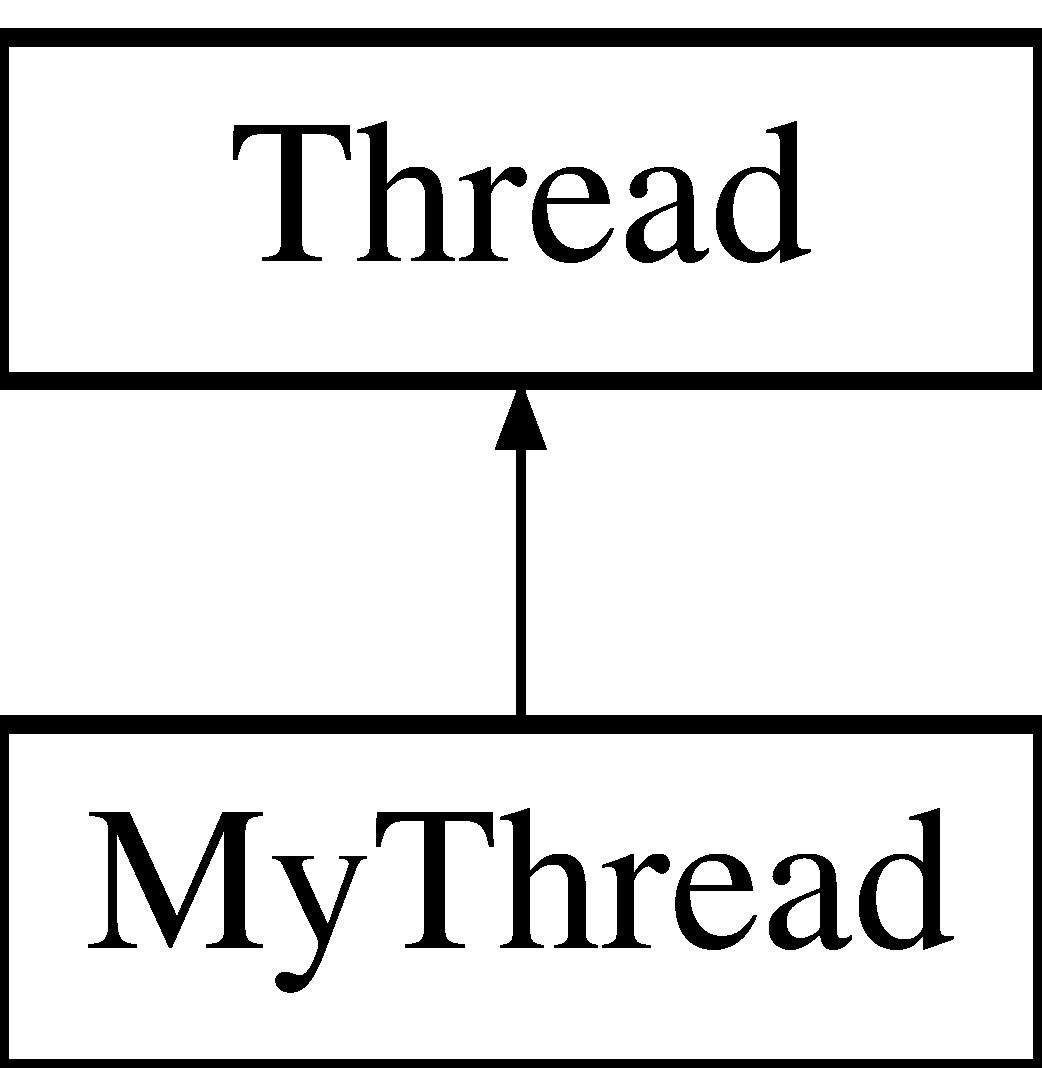
\includegraphics[height=2.000000cm]{class_my_thread}
\end{center}
\end{figure}
\subsection*{Public Member Functions}
\begin{DoxyCompactItemize}
\item 
\hypertarget{class_my_thread_a814ee8286a2406c3791ecaeb0eb042fb}{\hyperlink{class_my_thread_a814ee8286a2406c3791ecaeb0eb042fb}{My\-Thread} (queue$<$ \hyperlink{class_ball}{Ball} $\ast$ $>$ $\ast$)}\label{class_my_thread_a814ee8286a2406c3791ecaeb0eb042fb}

\begin{DoxyCompactList}\small\item\em Constructor. \end{DoxyCompactList}\item 
\hypertarget{class_my_thread_af6ab9a6669d1e1375f57bd35c8606ef1}{void \hyperlink{class_my_thread_af6ab9a6669d1e1375f57bd35c8606ef1}{set\-Queue} (queue$<$ \hyperlink{class_ball}{Ball} $\ast$ $>$ $\ast$)}\label{class_my_thread_af6ab9a6669d1e1375f57bd35c8606ef1}

\begin{DoxyCompactList}\small\item\em sets queue \end{DoxyCompactList}\item 
\hypertarget{class_my_thread_a9a3695f1605cea2664462cfe652b3f7b}{queue$<$ \hyperlink{class_ball}{Ball} $\ast$ $>$ $\ast$ \hyperlink{class_my_thread_a9a3695f1605cea2664462cfe652b3f7b}{get\-Queue} ()}\label{class_my_thread_a9a3695f1605cea2664462cfe652b3f7b}

\begin{DoxyCompactList}\small\item\em return queue \end{DoxyCompactList}\item 
\hypertarget{class_my_thread_a9289a1c82519f282f139f7d58a226a29}{void \hyperlink{class_my_thread_a9289a1c82519f282f139f7d58a226a29}{set\-Ball} (\hyperlink{class_ball}{Ball} $\ast$)}\label{class_my_thread_a9289a1c82519f282f139f7d58a226a29}

\begin{DoxyCompactList}\small\item\em sets the ball \end{DoxyCompactList}\item 
\hypertarget{class_my_thread_a06fb67170d01843c44cbea286c35546d}{\hyperlink{class_ball}{Ball} $\ast$ \hyperlink{class_my_thread_a06fb67170d01843c44cbea286c35546d}{get\-Ball} ()}\label{class_my_thread_a06fb67170d01843c44cbea286c35546d}

\begin{DoxyCompactList}\small\item\em return the ball \end{DoxyCompactList}\item 
\hypertarget{class_my_thread_a136aaa2ce85c45ad4a194a4b9baff8a1}{void $\ast$ \hyperlink{class_my_thread_a136aaa2ce85c45ad4a194a4b9baff8a1}{run} ()}\label{class_my_thread_a136aaa2ce85c45ad4a194a4b9baff8a1}

\begin{DoxyCompactList}\small\item\em function which runs when \hyperlink{class_thread_a7d563f3201d081af8cc24ea552c6a4e4}{start()} method of parent thread is called \end{DoxyCompactList}\end{DoxyCompactItemize}


\subsection{Detailed Description}
Extends the functionality of Class \hyperlink{class_thread}{Thread}. 

Extends \hyperlink{class_thread}{Thread} Class publicly 

The documentation for this class was generated from the following file\-:\begin{DoxyCompactItemize}
\item 
inc/My\-Thread.\-h\end{DoxyCompactItemize}

\hypertarget{class_particle}{\section{Particle Class Reference}
\label{class_particle}\index{Particle@{Particle}}
}


snow particles in background.  




{\ttfamily \#include $<$Particle.\-h$>$}

\subsection*{Public Member Functions}
\begin{DoxyCompactItemize}
\item 
\hypertarget{class_particle_a40f4c7e248029d72e7714b7802d5e5e1}{\hyperlink{class_particle_a40f4c7e248029d72e7714b7802d5e5e1}{Particle} ()}\label{class_particle_a40f4c7e248029d72e7714b7802d5e5e1}

\begin{DoxyCompactList}\small\item\em Constructor. \end{DoxyCompactList}\item 
\hypertarget{class_particle_ae965a3d556ffe29c80c97bbb18ab2372}{float \hyperlink{class_particle_ae965a3d556ffe29c80c97bbb18ab2372}{get\-Radius} ()}\label{class_particle_ae965a3d556ffe29c80c97bbb18ab2372}

\begin{DoxyCompactList}\small\item\em returns radius \end{DoxyCompactList}\item 
\hypertarget{class_particle_a49ad7061bf2b2362e36b8930a089c188}{void \hyperlink{class_particle_a49ad7061bf2b2362e36b8930a089c188}{set\-Radius} (float r)}\label{class_particle_a49ad7061bf2b2362e36b8930a089c188}

\begin{DoxyCompactList}\small\item\em sets the radius \end{DoxyCompactList}\item 
\hypertarget{class_particle_af3af4113b96e3ad0e079b5f815063321}{\hyperlink{global_8h_a62cc051caefbc94bc22d587ea537d9e8}{Three\-D} \hyperlink{class_particle_af3af4113b96e3ad0e079b5f815063321}{get\-Center} ()}\label{class_particle_af3af4113b96e3ad0e079b5f815063321}

\begin{DoxyCompactList}\small\item\em returns center \end{DoxyCompactList}\item 
\hypertarget{class_particle_a44a08aee886d132e353eea78c28fbbb4}{void \hyperlink{class_particle_a44a08aee886d132e353eea78c28fbbb4}{set\-Center} (float, float, float)}\label{class_particle_a44a08aee886d132e353eea78c28fbbb4}

\begin{DoxyCompactList}\small\item\em sets center \end{DoxyCompactList}\item 
\hypertarget{class_particle_adfd2e556815078426455241305abfb65}{\hyperlink{global_8h_a62cc051caefbc94bc22d587ea537d9e8}{Three\-D} \hyperlink{class_particle_adfd2e556815078426455241305abfb65}{get\-Velocity} ()}\label{class_particle_adfd2e556815078426455241305abfb65}

\begin{DoxyCompactList}\small\item\em returns velocity \end{DoxyCompactList}\item 
\hypertarget{class_particle_a91ad30eeee984cb8629f50eef6ab7f67}{void \hyperlink{class_particle_a91ad30eeee984cb8629f50eef6ab7f67}{set\-Velocity} (float, float, float)}\label{class_particle_a91ad30eeee984cb8629f50eef6ab7f67}

\begin{DoxyCompactList}\small\item\em sets velocity \end{DoxyCompactList}\item 
\hypertarget{class_particle_afedbd15814f27985408f520d9b3fd310}{void \hyperlink{class_particle_afedbd15814f27985408f520d9b3fd310}{draw\-P} ()}\label{class_particle_afedbd15814f27985408f520d9b3fd310}

\begin{DoxyCompactList}\small\item\em drawing utility function \end{DoxyCompactList}\item 
\hypertarget{class_particle_a61f4d976348cbb640287c2b85e01c3ce}{void \hyperlink{class_particle_a61f4d976348cbb640287c2b85e01c3ce}{move\-P} ()}\label{class_particle_a61f4d976348cbb640287c2b85e01c3ce}

\begin{DoxyCompactList}\small\item\em changes the position of snow particle \end{DoxyCompactList}\item 
\hypertarget{class_particle_a0df75e7ca5475b07c67746d7a7f41e22}{void \hyperlink{class_particle_a0df75e7ca5475b07c67746d7a7f41e22}{reset} ()}\label{class_particle_a0df75e7ca5475b07c67746d7a7f41e22}

\begin{DoxyCompactList}\small\item\em resets the position of snow particle \end{DoxyCompactList}\end{DoxyCompactItemize}


\subsection{Detailed Description}
snow particles in background. 

The documentation for this class was generated from the following file\-:\begin{DoxyCompactItemize}
\item 
inc/Particle.\-h\end{DoxyCompactItemize}

\hypertarget{class_theme}{\section{Theme Class Reference}
\label{class_theme}\index{Theme@{Theme}}
}


To store features of theme.  




{\ttfamily \#include $<$Theme.\-h$>$}

\subsection*{Public Member Functions}
\begin{DoxyCompactItemize}
\item 
\hypertarget{class_theme_a784069702b71190f6fb3f70362310789}{\hyperlink{class_theme_a784069702b71190f6fb3f70362310789}{Theme} ()}\label{class_theme_a784069702b71190f6fb3f70362310789}

\begin{DoxyCompactList}\small\item\em \hyperlink{class_theme}{Theme} with default settings. \end{DoxyCompactList}\end{DoxyCompactItemize}
\subsection*{Public Attributes}
\begin{DoxyCompactItemize}
\item 
\hypertarget{class_theme_a486d4eda08361ce1cb61a8f93dda8884}{\hyperlink{global_8h_aae4bd90e8e9fa4cdfa4e10e3494f755b}{Color} \hyperlink{class_theme_a486d4eda08361ce1cb61a8f93dda8884}{background}}\label{class_theme_a486d4eda08361ce1cb61a8f93dda8884}

\begin{DoxyCompactList}\small\item\em Background color. \end{DoxyCompactList}\item 
\hypertarget{class_theme_abb2caa63e627e47504fed37ec34023d0}{\hyperlink{global_8h_aae4bd90e8e9fa4cdfa4e10e3494f755b}{Color} \hyperlink{class_theme_abb2caa63e627e47504fed37ec34023d0}{clr} \mbox{[}3\mbox{]}}\label{class_theme_abb2caa63e627e47504fed37ec34023d0}

\begin{DoxyCompactList}\small\item\em Lighting color. \end{DoxyCompactList}\item 
\hypertarget{class_theme_ab948e47a7f15fe10a4a8c9794af91ac3}{\hyperlink{global_8h_a62cc051caefbc94bc22d587ea537d9e8}{Three\-D} \hyperlink{class_theme_ab948e47a7f15fe10a4a8c9794af91ac3}{pos} \mbox{[}3\mbox{]}}\label{class_theme_ab948e47a7f15fe10a4a8c9794af91ac3}

\begin{DoxyCompactList}\small\item\em Lights position. \end{DoxyCompactList}\item 
\hypertarget{class_theme_a2e2b3f1e6b563c30aecf9e41c5f512af}{bool \hyperlink{class_theme_a2e2b3f1e6b563c30aecf9e41c5f512af}{is\-Light} \mbox{[}4\mbox{]}}\label{class_theme_a2e2b3f1e6b563c30aecf9e41c5f512af}

\begin{DoxyCompactList}\small\item\em Enable/\-Disable Light. \end{DoxyCompactList}\item 
\hypertarget{class_theme_af6416fd1e8cace10a0a4d436ad5bd7c3}{string \hyperlink{class_theme_af6416fd1e8cace10a0a4d436ad5bd7c3}{image}}\label{class_theme_af6416fd1e8cace10a0a4d436ad5bd7c3}

\begin{DoxyCompactList}\small\item\em Background \hyperlink{class_image}{Image}. \end{DoxyCompactList}\end{DoxyCompactItemize}


\subsection{Detailed Description}
To store features of theme. 

Changes in this and \hyperlink{theme_reader_8h}{should be in sync }

The documentation for this class was generated from the following file\-:\begin{DoxyCompactItemize}
\item 
inc/Theme.\-h\end{DoxyCompactItemize}

\hypertarget{class_thread}{\section{Thread Class Reference}
\label{class_thread}\index{Thread@{Thread}}
}


Class to be inherited by \hyperlink{class_my_thread}{My\-Thread}.  




{\ttfamily \#include $<$thr.\-h$>$}

Inheritance diagram for Thread\-:\begin{figure}[H]
\begin{center}
\leavevmode
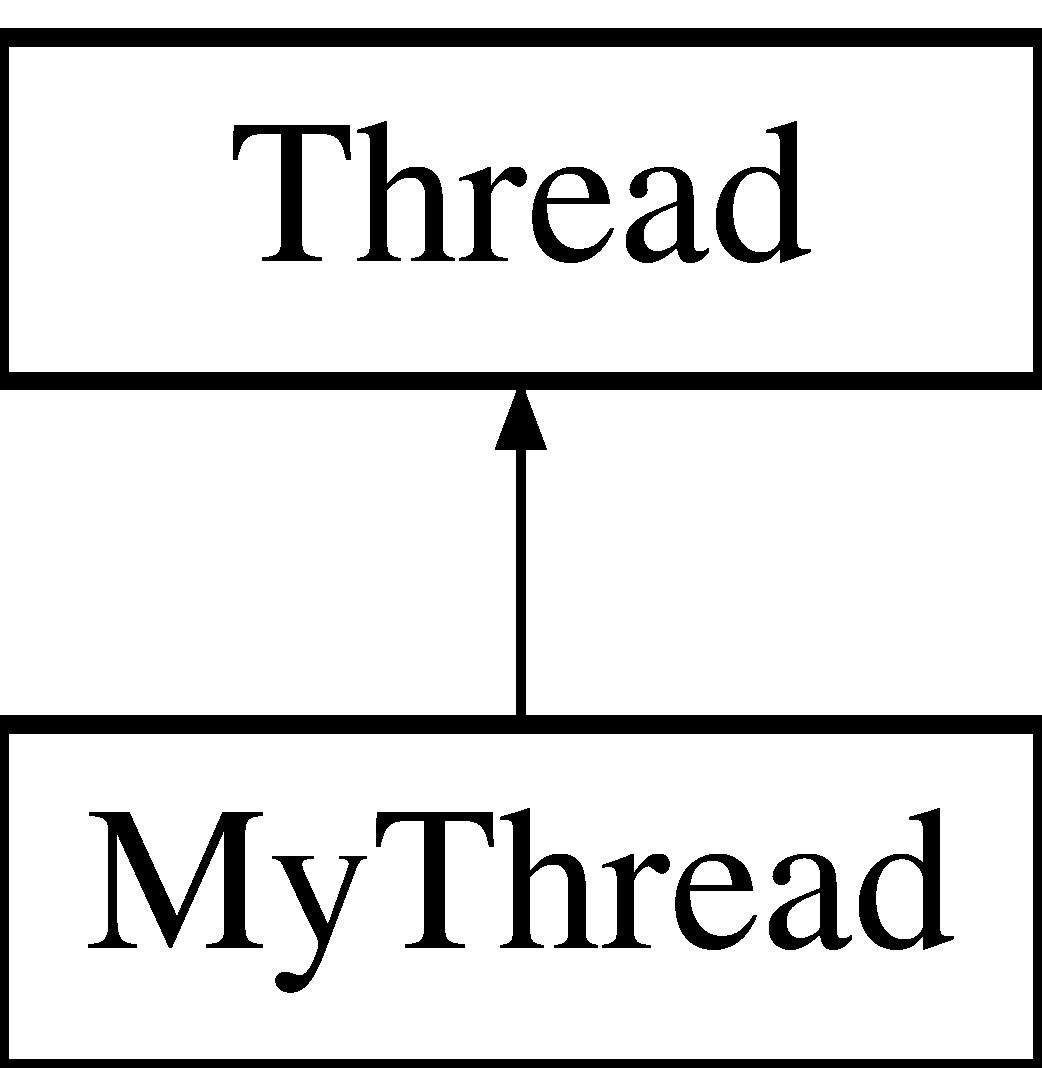
\includegraphics[height=2.000000cm]{class_thread}
\end{center}
\end{figure}
\subsection*{Public Member Functions}
\begin{DoxyCompactItemize}
\item 
\hypertarget{class_thread_a95c703fb8f2f27cb64f475a8c940864a}{\hyperlink{class_thread_a95c703fb8f2f27cb64f475a8c940864a}{Thread} ()}\label{class_thread_a95c703fb8f2f27cb64f475a8c940864a}

\begin{DoxyCompactList}\small\item\em Constructor. \end{DoxyCompactList}\item 
\hypertarget{class_thread_a37d9edd3a1a776cbc27dedff949c9726}{\hyperlink{class_thread_a37d9edd3a1a776cbc27dedff949c9726}{$\sim$\-Thread} ()}\label{class_thread_a37d9edd3a1a776cbc27dedff949c9726}

\begin{DoxyCompactList}\small\item\em Destructor. \end{DoxyCompactList}\item 
\hypertarget{class_thread_a7d563f3201d081af8cc24ea552c6a4e4}{int \hyperlink{class_thread_a7d563f3201d081af8cc24ea552c6a4e4}{start} ()}\label{class_thread_a7d563f3201d081af8cc24ea552c6a4e4}

\begin{DoxyCompactList}\small\item\em creates a thread and calls run() method \end{DoxyCompactList}\item 
\hypertarget{class_thread_a7c3b04b32b4327923cc4c9553a403e32}{int \hyperlink{class_thread_a7c3b04b32b4327923cc4c9553a403e32}{join} ()}\label{class_thread_a7c3b04b32b4327923cc4c9553a403e32}

\begin{DoxyCompactList}\small\item\em joins the thread \end{DoxyCompactList}\item 
\hypertarget{class_thread_a2a08036a4598cfc554114fee9d0e8485}{int \hyperlink{class_thread_a2a08036a4598cfc554114fee9d0e8485}{detach} ()}\label{class_thread_a2a08036a4598cfc554114fee9d0e8485}

\begin{DoxyCompactList}\small\item\em detaches the thread \end{DoxyCompactList}\item 
\hypertarget{class_thread_ad4242a739c70bd1fe6b9c6e208714310}{pthread\-\_\-t \hyperlink{class_thread_ad4242a739c70bd1fe6b9c6e208714310}{self} ()}\label{class_thread_ad4242a739c70bd1fe6b9c6e208714310}

\begin{DoxyCompactList}\small\item\em return thread Id \end{DoxyCompactList}\item 
\hypertarget{class_thread_a0ceaa28981eacf1051845542053d82b6}{virtual void $\ast$ {\bfseries run} ()=0}\label{class_thread_a0ceaa28981eacf1051845542053d82b6}

\end{DoxyCompactItemize}


\subsection{Detailed Description}
Class to be inherited by \hyperlink{class_my_thread}{My\-Thread}. 

The documentation for this class was generated from the following file\-:\begin{DoxyCompactItemize}
\item 
inc/thr.\-h\end{DoxyCompactItemize}

\hypertarget{class_wall}{\section{Wall Class Reference}
\label{class_wall}\index{Wall@{Wall}}
}


\hyperlink{class_wall}{Wall} object to define boundaries of window/box.  




{\ttfamily \#include $<$Wall.\-h$>$}

\subsection*{Public Member Functions}
\begin{DoxyCompactItemize}
\item 
\hypertarget{class_wall_a12dc41bc7bc045c55ec1034a43e52043}{\hyperlink{class_wall_a12dc41bc7bc045c55ec1034a43e52043}{Wall} ()}\label{class_wall_a12dc41bc7bc045c55ec1034a43e52043}

\begin{DoxyCompactList}\small\item\em Constructor. \end{DoxyCompactList}\item 
\hypertarget{class_wall_ae4f555d738a794750a3a3eee13224aa6}{\hyperlink{class_wall_ae4f555d738a794750a3a3eee13224aa6}{Wall} (Plane\-Type, float)}\label{class_wall_ae4f555d738a794750a3a3eee13224aa6}

\begin{DoxyCompactList}\small\item\em Creates wall with at given positon of given type. \end{DoxyCompactList}\item 
\hypertarget{class_wall_a5078f7c871c757e37d3604dc91194058}{Plane\-Type \hyperlink{class_wall_a5078f7c871c757e37d3604dc91194058}{get\-Plane} () const }\label{class_wall_a5078f7c871c757e37d3604dc91194058}

\begin{DoxyCompactList}\small\item\em Returns type of the plane. \end{DoxyCompactList}\item 
\hypertarget{class_wall_aa5842de4210e80f6bd539a3438d76458}{float \hyperlink{class_wall_aa5842de4210e80f6bd539a3438d76458}{get\-Position} () const }\label{class_wall_aa5842de4210e80f6bd539a3438d76458}

\begin{DoxyCompactList}\small\item\em Returns the position of the plane. \end{DoxyCompactList}\item 
\hypertarget{class_wall_add5e93f662291366050b73dec61ac7cf}{void \hyperlink{class_wall_add5e93f662291366050b73dec61ac7cf}{set\-Position} (float)}\label{class_wall_add5e93f662291366050b73dec61ac7cf}

\begin{DoxyCompactList}\small\item\em Sets the position of the plane. \end{DoxyCompactList}\end{DoxyCompactItemize}


\subsection{Detailed Description}
\hyperlink{class_wall}{Wall} object to define boundaries of window/box. 

The documentation for this class was generated from the following file\-:\begin{DoxyCompactItemize}
\item 
inc/Wall.\-h\end{DoxyCompactItemize}

\chapter{File Documentation}
\hypertarget{_collision_8h}{\section{inc/\-Collision.h File Reference}
\label{_collision_8h}\index{inc/\-Collision.\-h@{inc/\-Collision.\-h}}
}
{\ttfamily \#include \char`\"{}Wall.\-h\char`\"{}}\\*
{\ttfamily \#include \char`\"{}Ball.\-h\char`\"{}}\\*
\subsection*{Functions}
\begin{DoxyCompactItemize}
\item 
\hypertarget{_collision_8h_a6a1cf3bca9df4b9cdff131b864270b38}{void \hyperlink{_collision_8h_a6a1cf3bca9df4b9cdff131b864270b38}{check\-\_\-\-Collision\-\_\-\-With\-\_\-\-Wall} (\hyperlink{class_ball}{Ball} \&, \hyperlink{class_wall}{Wall} \&)}\label{_collision_8h_a6a1cf3bca9df4b9cdff131b864270b38}

\begin{DoxyCompactList}\small\item\em Checks for a possible collision of a ball with a wall and accordingly update the velocity. \end{DoxyCompactList}\item 
\hypertarget{_collision_8h_a118ccd139751c26b12a82ae89635ad5d}{void \hyperlink{_collision_8h_a118ccd139751c26b12a82ae89635ad5d}{check\-\_\-\-Collision\-\_\-\-With\-\_\-\-Ball} (\hyperlink{class_ball}{Ball} \&, \hyperlink{class_ball}{Ball} \&)}\label{_collision_8h_a118ccd139751c26b12a82ae89635ad5d}

\begin{DoxyCompactList}\small\item\em Checks for a possible collision of two balls with each other and accordingly update the velocities of both the balls using their respective mutexes. \end{DoxyCompactList}\end{DoxyCompactItemize}


\subsection{Detailed Description}
Functions for maintaining the physics of the system. \par
 All the collisions are elastic. 
\hypertarget{global_8h}{\section{inc/global.h File Reference}
\label{global_8h}\index{inc/global.\-h@{inc/global.\-h}}
}
\subsection*{Classes}
\begin{DoxyCompactItemize}
\item 
struct \hyperlink{struct_my_struct}{My\-Struct}
\begin{DoxyCompactList}\small\item\em To store three dimensional variables like position, velocity, etc. \end{DoxyCompactList}\item 
struct \hyperlink{struct_my_color}{My\-Color}
\begin{DoxyCompactList}\small\item\em To store the color attribute in R\-G\-B format. \end{DoxyCompactList}\end{DoxyCompactItemize}
\subsection*{Typedefs}
\begin{DoxyCompactItemize}
\item 
\hypertarget{global_8h_a62cc051caefbc94bc22d587ea537d9e8}{typedef struct \hyperlink{struct_my_struct}{My\-Struct} \hyperlink{global_8h_a62cc051caefbc94bc22d587ea537d9e8}{Three\-D}}\label{global_8h_a62cc051caefbc94bc22d587ea537d9e8}

\begin{DoxyCompactList}\small\item\em To store three dimensional variables like position, velocity, etc. \end{DoxyCompactList}\item 
\hypertarget{global_8h_aae4bd90e8e9fa4cdfa4e10e3494f755b}{typedef struct \hyperlink{struct_my_color}{My\-Color} \hyperlink{global_8h_aae4bd90e8e9fa4cdfa4e10e3494f755b}{Color}}\label{global_8h_aae4bd90e8e9fa4cdfa4e10e3494f755b}

\begin{DoxyCompactList}\small\item\em To store the color attribute in R\-G\-B format. \end{DoxyCompactList}\end{DoxyCompactItemize}


\subsection{Detailed Description}
Useful Structures are defined here. 
\hypertarget{_g_u_i_8h}{\section{inc/\-G\-U\-I.h File Reference}
\label{_g_u_i_8h}\index{inc/\-G\-U\-I.\-h@{inc/\-G\-U\-I.\-h}}
}
{\ttfamily \#include $<$G\-L/glut.\-h$>$}\\*
{\ttfamily \#include $<$G\-L/glui.\-h$>$}\\*
{\ttfamily \#include \char`\"{}image\-Load.\-h\char`\"{}}\\*
\subsection*{Functions}
\begin{DoxyCompactItemize}
\item 
\hypertarget{_g_u_i_8h_ac74398020ba83af6fd9a2a802fecc19e}{void \hyperlink{_g_u_i_8h_ac74398020ba83af6fd9a2a802fecc19e}{handle\-Mouse} (int, int, int, int)}\label{_g_u_i_8h_ac74398020ba83af6fd9a2a802fecc19e}

\begin{DoxyCompactList}\small\item\em glut\-Mouse\-Func \end{DoxyCompactList}\item 
\hypertarget{_g_u_i_8h_a2fac10444592108d0a25618404d9ffb9}{void \hyperlink{_g_u_i_8h_a2fac10444592108d0a25618404d9ffb9}{handle\-Resize} (int, int)}\label{_g_u_i_8h_a2fac10444592108d0a25618404d9ffb9}

\begin{DoxyCompactList}\small\item\em glut\-Reshape\-Func \end{DoxyCompactList}\item 
\hypertarget{_g_u_i_8h_aa420ffe7fa846fa65172f2c868e65c3b}{void \hyperlink{_g_u_i_8h_aa420ffe7fa846fa65172f2c868e65c3b}{handle\-Keypress} (unsigned char, int, int)}\label{_g_u_i_8h_aa420ffe7fa846fa65172f2c868e65c3b}

\begin{DoxyCompactList}\small\item\em glut\-Keyboard\-Func \end{DoxyCompactList}\item 
\hypertarget{_g_u_i_8h_a05c3c225665f78f6c21b2a2789f7bac9}{G\-Luint \hyperlink{_g_u_i_8h_a05c3c225665f78f6c21b2a2789f7bac9}{load\-Texture} (\hyperlink{class_image}{Image} $\ast$)}\label{_g_u_i_8h_a05c3c225665f78f6c21b2a2789f7bac9}

\begin{DoxyCompactList}\small\item\em loads texture from an \hyperlink{class_image}{Image} \end{DoxyCompactList}\item 
\hypertarget{_g_u_i_8h_a8b37041e24634374ba92c3779498778d}{void \hyperlink{_g_u_i_8h_a8b37041e24634374ba92c3779498778d}{draw\-Box} ()}\label{_g_u_i_8h_a8b37041e24634374ba92c3779498778d}

\begin{DoxyCompactList}\small\item\em draws a 3\-D box at boundaries of balls i.\-e. walls \end{DoxyCompactList}\item 
\hypertarget{_g_u_i_8h_a1dad859c998887477cd90323a027b8c6}{void \hyperlink{_g_u_i_8h_a1dad859c998887477cd90323a027b8c6}{draw\-Scene} ()}\label{_g_u_i_8h_a1dad859c998887477cd90323a027b8c6}

\begin{DoxyCompactList}\small\item\em glut\-Draw\-Func \end{DoxyCompactList}\item 
\hypertarget{_g_u_i_8h_a17a53fe9e683b81bdc7618f88b8b8502}{void \hyperlink{_g_u_i_8h_a17a53fe9e683b81bdc7618f88b8b8502}{init\-Rendering} ()}\label{_g_u_i_8h_a17a53fe9e683b81bdc7618f88b8b8502}

\begin{DoxyCompactList}\small\item\em initialize the graphics rendering \end{DoxyCompactList}\item 
\hypertarget{_g_u_i_8h_a9c62bb6d630b583e53331bedf18b051b}{void \hyperlink{_g_u_i_8h_a9c62bb6d630b583e53331bedf18b051b}{update} (int)}\label{_g_u_i_8h_a9c62bb6d630b583e53331bedf18b051b}

\begin{DoxyCompactList}\small\item\em glut\-Timer\-Func \end{DoxyCompactList}\end{DoxyCompactItemize}


\subsection{Detailed Description}
open\-G\-L functions are maintained in this seperate file. \par
 Any changes regarding graphics rendering should be made here. 
\hypertarget{mainw_8h}{\section{inc/mainw.h File Reference}
\label{mainw_8h}\index{inc/mainw.\-h@{inc/mainw.\-h}}
}
{\ttfamily \#include $<$G\-L/glut.\-h$>$}\\*
{\ttfamily \#include $<$G\-L/glui.\-h$>$}\\*
{\ttfamily \#include $<$queue$>$}\\*
{\ttfamily \#include $<$vector$>$}\\*
{\ttfamily \#include $<$utility$>$}\\*
{\ttfamily \#include \char`\"{}Ball.\-h\char`\"{}}\\*
{\ttfamily \#include \char`\"{}My\-Thread.\-h\char`\"{}}\\*
{\ttfamily \#include \char`\"{}Wall.\-h\char`\"{}}\\*
{\ttfamily \#include \char`\"{}Theme.\-h\char`\"{}}\\*
{\ttfamily \#include \char`\"{}image\-Load.\-h\char`\"{}}\\*
{\ttfamily \#include \char`\"{}Particle.\-h\char`\"{}}\\*
\subsection*{Variables}
\begin{DoxyCompactItemize}
\item 
\hypertarget{mainw_8h_a1b2c942e430336bbd74c098cf6333fbc}{float {\bfseries A\-L\-P\-H\-A}}\label{mainw_8h_a1b2c942e430336bbd74c098cf6333fbc}

\item 
\hypertarget{mainw_8h_a4ebf53356b6bbe17fbe3a03d3fa79e87}{float {\bfseries rotate}}\label{mainw_8h_a4ebf53356b6bbe17fbe3a03d3fa79e87}

\item 
\hypertarget{mainw_8h_a14924d7fdcf8a844929f9ca2ad4dacfe}{int {\bfseries number\-\_\-of\-\_\-balls}}\label{mainw_8h_a14924d7fdcf8a844929f9ca2ad4dacfe}

\item 
\hypertarget{mainw_8h_ae1cff101bb582ade8865de9b2b33bf2f}{vector$<$ \hyperlink{class_my_thread}{My\-Thread} $\ast$ $>$ {\bfseries threads}}\label{mainw_8h_ae1cff101bb582ade8865de9b2b33bf2f}

\item 
\hypertarget{mainw_8h_ad409cd5bb7aa5b217a2cf80cdd3e886c}{float {\bfseries wide\-Angle}}\label{mainw_8h_ad409cd5bb7aa5b217a2cf80cdd3e886c}

\item 
\hypertarget{mainw_8h_a207ad05f99cc72068a92358861ff5e71}{float {\bfseries ratio}}\label{mainw_8h_a207ad05f99cc72068a92358861ff5e71}

\item 
\hypertarget{mainw_8h_aca33f926b061680d857699a22f676418}{int {\bfseries window\-\_\-height}}\label{mainw_8h_aca33f926b061680d857699a22f676418}

\item 
\hypertarget{mainw_8h_a0e2e740afd510cfe652a1836ffbad209}{int {\bfseries window\-\_\-width}}\label{mainw_8h_a0e2e740afd510cfe652a1836ffbad209}

\item 
\hypertarget{mainw_8h_a9a57f322df958dc574c9843c6ab4b1c2}{float {\bfseries angle\-X}}\label{mainw_8h_a9a57f322df958dc574c9843c6ab4b1c2}

\item 
\hypertarget{mainw_8h_adb82b6f9a59b4ebab80b0ea796dbe066}{float {\bfseries angle\-Y}}\label{mainw_8h_adb82b6f9a59b4ebab80b0ea796dbe066}

\item 
\hypertarget{mainw_8h_aa67cf2b62fb9fc5f61976d3d3984975e}{float {\bfseries angle\-Z}}\label{mainw_8h_aa67cf2b62fb9fc5f61976d3d3984975e}

\item 
\hypertarget{mainw_8h_a40752b82e16b22820b34c2a88deebfec}{int {\bfseries border\-Number}}\label{mainw_8h_a40752b82e16b22820b34c2a88deebfec}

\item 
\hypertarget{mainw_8h_ab707e2b937986a02db21b03d7b60d540}{float {\bfseries view\-Distance}}\label{mainw_8h_ab707e2b937986a02db21b03d7b60d540}

\item 
\hypertarget{mainw_8h_a18f6bf0689a7859143bc316226be4c96}{G\-Luint {\bfseries t1}}\label{mainw_8h_a18f6bf0689a7859143bc316226be4c96}

\item 
\hypertarget{mainw_8h_a6efda4056e913314bf3c5066749b1bdf}{G\-Luint {\bfseries tex3d}}\label{mainw_8h_a6efda4056e913314bf3c5066749b1bdf}

\item 
\hypertarget{mainw_8h_ad7fcfe6c2accb828df3b77287cacc471}{G\-Luint {\bfseries wall\-\_\-tex}}\label{mainw_8h_ad7fcfe6c2accb828df3b77287cacc471}

\item 
\hypertarget{mainw_8h_abed43ec97a78abdf5acf6e29033844d4}{G\-L\-Uquadric $\ast$ {\bfseries quad}}\label{mainw_8h_abed43ec97a78abdf5acf6e29033844d4}

\item 
\hypertarget{mainw_8h_a52c13b1b02a8dc4f543da3796c0ae55c}{G\-Luint {\bfseries \-\_\-texture\-Id}}\label{mainw_8h_a52c13b1b02a8dc4f543da3796c0ae55c}

\item 
\hypertarget{mainw_8h_ab2126459af6615dcd7a7020f7bd653f2}{vector$<$ \hyperlink{class_theme}{Theme} $\ast$ $>$ {\bfseries themes}}\label{mainw_8h_ab2126459af6615dcd7a7020f7bd653f2}

\item 
\hypertarget{mainw_8h_a80f3e70d8eec5fe2e2934724c9b0d54e}{\hyperlink{class_theme}{Theme} $\ast$ {\bfseries cur\-Theme}}\label{mainw_8h_a80f3e70d8eec5fe2e2934724c9b0d54e}

\item 
\hypertarget{mainw_8h_abc92767291dd1138ad4dafb966db51bc}{\hyperlink{class_wall}{Wall} {\bfseries wall\-\_\-x}}\label{mainw_8h_abc92767291dd1138ad4dafb966db51bc}

\item 
\hypertarget{mainw_8h_a08416cb47f09a51448190f49b269d839}{\hyperlink{class_wall}{Wall} {\bfseries wall\-\_\-y}}\label{mainw_8h_a08416cb47f09a51448190f49b269d839}

\item 
\hypertarget{mainw_8h_a874f8e54d97a5f0efbad24116907d5c2}{\hyperlink{class_wall}{Wall} {\bfseries wall\-\_\-z}}\label{mainw_8h_a874f8e54d97a5f0efbad24116907d5c2}

\item 
\hypertarget{mainw_8h_a83632b0b4225896cb4b281c8481913bf}{\hyperlink{class_particle}{Particle} $\ast$ {\bfseries particles}}\label{mainw_8h_a83632b0b4225896cb4b281c8481913bf}

\end{DoxyCompactItemize}


\subsection{Detailed Description}
File containing global variables to be used in other files/classes \par
 
\hypertarget{_my_defines_8h}{\section{inc/\-My\-Defines.h File Reference}
\label{_my_defines_8h}\index{inc/\-My\-Defines.\-h@{inc/\-My\-Defines.\-h}}
}
\subsection*{Macros}
\begin{DoxyCompactItemize}
\item 
\hypertarget{group___d_e_f_i_n_e_ga9d7f8570df9132e87f4e56209206f13a}{\#define \hyperlink{group___d_e_f_i_n_e_ga9d7f8570df9132e87f4e56209206f13a}{M\-A\-X\-\_\-\-N\-U\-M\-\_\-\-B\-A\-L\-L\-S}~1000}\label{group___d_e_f_i_n_e_ga9d7f8570df9132e87f4e56209206f13a}

\begin{DoxyCompactList}\small\item\em Maximum number of balls possible on screen. \end{DoxyCompactList}\item 
\hypertarget{group___d_e_f_i_n_e_ga238c53c07c05119952391d18f00bf3bb}{\#define \hyperlink{group___d_e_f_i_n_e_ga238c53c07c05119952391d18f00bf3bb}{U\-P\-D\-A\-T\-E\-\_\-\-T\-I\-M\-E\-R}~20}\label{group___d_e_f_i_n_e_ga238c53c07c05119952391d18f00bf3bb}

\begin{DoxyCompactList}\small\item\em Minimum time before next \hyperlink{_g_u_i_8h_a9c62bb6d630b583e53331bedf18b051b}{update(int)} function is called. \end{DoxyCompactList}\item 
\hypertarget{group___d_e_f_i_n_e_ga030ebc610fddb0a18d62829ab376bf85}{\#define \hyperlink{group___d_e_f_i_n_e_ga030ebc610fddb0a18d62829ab376bf85}{D\-E\-F\-A\-U\-L\-T\-\_\-\-W\-I\-N\-D\-O\-W\-\_\-\-H\-E\-I\-G\-H\-T}~1056}\label{group___d_e_f_i_n_e_ga030ebc610fddb0a18d62829ab376bf85}

\begin{DoxyCompactList}\small\item\em Initial height of window. \end{DoxyCompactList}\item 
\hypertarget{group___d_e_f_i_n_e_ga6ca4df6b9e1495a80a2929a5187cb9b9}{\#define \hyperlink{group___d_e_f_i_n_e_ga6ca4df6b9e1495a80a2929a5187cb9b9}{D\-E\-F\-A\-U\-L\-T\-\_\-\-W\-I\-N\-D\-O\-W\-\_\-\-W\-I\-D\-T\-H}~1855}\label{group___d_e_f_i_n_e_ga6ca4df6b9e1495a80a2929a5187cb9b9}

\begin{DoxyCompactList}\small\item\em Initial width of window. \end{DoxyCompactList}\item 
\hypertarget{group___d_e_f_i_n_e_ga624e1e19728aaa9abcfb678c6025e38f}{\#define \hyperlink{group___d_e_f_i_n_e_ga624e1e19728aaa9abcfb678c6025e38f}{D\-E\-F\-A\-U\-L\-T\-\_\-\-W\-I\-N\-D\-O\-W\-\_\-\-D\-E\-P\-T\-H}~600}\label{group___d_e_f_i_n_e_ga624e1e19728aaa9abcfb678c6025e38f}

\begin{DoxyCompactList}\small\item\em Initial Depth of box (in 3\-D view) \end{DoxyCompactList}\item 
\hypertarget{group___d_e_f_i_n_e_gae18610b134c10d11e590b789ca741d61}{\#define \hyperlink{group___d_e_f_i_n_e_gae18610b134c10d11e590b789ca741d61}{T\-I\-M\-E\-\_\-\-L\-A\-G}~50}\label{group___d_e_f_i_n_e_gae18610b134c10d11e590b789ca741d61}

\begin{DoxyCompactList}\small\item\em Time after which succesive balls enter the window. \end{DoxyCompactList}\item 
\hypertarget{group___d_e_f_i_n_e_gaddd7cbe43c46d853f4128514b916b393}{\#define \hyperlink{group___d_e_f_i_n_e_gaddd7cbe43c46d853f4128514b916b393}{N\-U\-M\-\_\-\-S\-E\-G\-M\-E\-N\-T\-S}~100}\label{group___d_e_f_i_n_e_gaddd7cbe43c46d853f4128514b916b393}

\begin{DoxyCompactList}\small\item\em Number of segment along and around z-\/axis of sphere. \end{DoxyCompactList}\item 
\hypertarget{group___d_e_f_i_n_e_ga75e5e541dc25d8b29e327598825ea914}{\#define \hyperlink{group___d_e_f_i_n_e_ga75e5e541dc25d8b29e327598825ea914}{L\-I\-M\-I\-T\-\_\-\-W}~500}\label{group___d_e_f_i_n_e_ga75e5e541dc25d8b29e327598825ea914}

\begin{DoxyCompactList}\small\item\em Minimum width of window. \end{DoxyCompactList}\item 
\hypertarget{group___d_e_f_i_n_e_ga69e965de5fac4f8e733454dc17872c35}{\#define \hyperlink{group___d_e_f_i_n_e_ga69e965de5fac4f8e733454dc17872c35}{L\-I\-M\-I\-T\-\_\-\-H}~500}\label{group___d_e_f_i_n_e_ga69e965de5fac4f8e733454dc17872c35}

\begin{DoxyCompactList}\small\item\em Minimum height of window. \end{DoxyCompactList}\item 
\hypertarget{group___d_e_f_i_n_e_ga598a3330b3c21701223ee0ca14316eca}{\#define \hyperlink{group___d_e_f_i_n_e_ga598a3330b3c21701223ee0ca14316eca}{P\-I}~3.\-1415926f}\label{group___d_e_f_i_n_e_ga598a3330b3c21701223ee0ca14316eca}

\begin{DoxyCompactList}\small\item\em Value of \href{http://en.wikipedia.org/wiki/Pi}{\tt P\-I} \end{DoxyCompactList}\item 
\hypertarget{group___d_e_f_i_n_e_gab93c45e95c408a9ab17a501275bc62fb}{\#define \hyperlink{group___d_e_f_i_n_e_gab93c45e95c408a9ab17a501275bc62fb}{C\-H\-A\-N\-G\-E\-\_\-\-F\-A\-C\-T\-O\-R}~1.\-2f}\label{group___d_e_f_i_n_e_gab93c45e95c408a9ab17a501275bc62fb}

\begin{DoxyCompactList}\small\item\em Factor by which speed is increased/decreased on a single click on increase/decrease buttons. \end{DoxyCompactList}\item 
\hypertarget{group___d_e_f_i_n_e_ga1316e2e8c9434231dfeeb62dff9c7252}{\#define \hyperlink{group___d_e_f_i_n_e_ga1316e2e8c9434231dfeeb62dff9c7252}{M\-A\-X\-\_\-\-S\-P\-L\-I\-T\-S}~7;}\label{group___d_e_f_i_n_e_ga1316e2e8c9434231dfeeb62dff9c7252}

\begin{DoxyCompactList}\small\item\em Max number of smaller balls on splitting a ball. \end{DoxyCompactList}\item 
\hypertarget{group___d_e_f_i_n_e_gaeb58f5e1ee76192500493fe94c3ab80b}{\#define \hyperlink{group___d_e_f_i_n_e_gaeb58f5e1ee76192500493fe94c3ab80b}{z\-Distance}~15.\-0f}\label{group___d_e_f_i_n_e_gaeb58f5e1ee76192500493fe94c3ab80b}

\begin{DoxyCompactList}\small\item\em Default view distance from the plane of drawing. \end{DoxyCompactList}\item 
\hypertarget{group___d_e_f_i_n_e_ga943f07034774ef1261d62cd0d3d1fec9}{\#define \hyperlink{group___d_e_f_i_n_e_ga943f07034774ef1261d62cd0d3d1fec9}{D\-T}~0.\-5f}\label{group___d_e_f_i_n_e_ga943f07034774ef1261d62cd0d3d1fec9}

\begin{DoxyCompactList}\small\item\em Time for which position of ball is changed in each update call. \end{DoxyCompactList}\item 
\hypertarget{group___d_e_f_i_n_e_ga75cbc112dce4b21c13fe7bb671accab1}{\#define \hyperlink{group___d_e_f_i_n_e_ga75cbc112dce4b21c13fe7bb671accab1}{N\-U\-M\-\_\-\-P\-A\-R\-T\-I\-C\-L\-E\-S}~1000}\label{group___d_e_f_i_n_e_ga75cbc112dce4b21c13fe7bb671accab1}

\begin{DoxyCompactList}\small\item\em Number of snow particles in the background. \end{DoxyCompactList}\end{DoxyCompactItemize}


\subsection{Detailed Description}
All the constants are defined here in seperate file. 
\hypertarget{_my_enums_8h}{\section{inc/\-My\-Enums.h File Reference}
\label{_my_enums_8h}\index{inc/\-My\-Enums.\-h@{inc/\-My\-Enums.\-h}}
}
\subsection*{Enumerations}
\begin{DoxyCompactItemize}
\item 
enum {\bfseries Game\-State} \{ {\bfseries P\-L\-A\-Y}, 
{\bfseries P\-A\-U\-S\-E}
 \}
\item 
enum {\bfseries Select} \{ {\bfseries Y\-E\-S}, 
{\bfseries N\-O}
 \}
\end{DoxyCompactItemize}
\subsection*{Variables}
\begin{DoxyCompactItemize}
\item 
\hypertarget{group___t_y_p_e_d_e_f_s_ga2706ed05d331ef3b53c728a6868bda26}{Game\-State {\bfseries game\-State}}\label{group___t_y_p_e_d_e_f_s_ga2706ed05d331ef3b53c728a6868bda26}

\item 
\hypertarget{group___t_y_p_e_d_e_f_s_gaedf00c9118f2afc5321a133ab13a771a}{Select {\bfseries border}}\label{group___t_y_p_e_d_e_f_s_gaedf00c9118f2afc5321a133ab13a771a}

\item 
\hypertarget{group___t_y_p_e_d_e_f_s_gab8182ca59816bb30f7ebe46b37615cf7}{Select {\bfseries show\-Menu}}\label{group___t_y_p_e_d_e_f_s_gab8182ca59816bb30f7ebe46b37615cf7}

\item 
\hypertarget{group___t_y_p_e_d_e_f_s_gacaced8dd742dbb5fa7e0e8bf6061e393}{Select {\bfseries enable3\-D}}\label{group___t_y_p_e_d_e_f_s_gacaced8dd742dbb5fa7e0e8bf6061e393}

\end{DoxyCompactItemize}


\subsection{Detailed Description}
Enums are defined in this seperate file. 
\hypertarget{sub_menu_8h}{\section{inc/sub\-Menu.h File Reference}
\label{sub_menu_8h}\index{inc/sub\-Menu.\-h@{inc/sub\-Menu.\-h}}
}
{\ttfamily \#include $<$G\-L/glut.\-h$>$}\\*
{\ttfamily \#include $<$G\-L/glui.\-h$>$}\\*
{\ttfamily \#include $<$string.\-h$>$}\\*
\subsection*{Functions}
\begin{DoxyCompactItemize}
\item 
\hypertarget{sub_menu_8h_a1ab2e419a91c117b5ff3f5e75445d1ad}{void \hyperlink{sub_menu_8h_a1ab2e419a91c117b5ff3f5e75445d1ad}{my\-Glut\-Idle} (void)}\label{sub_menu_8h_a1ab2e419a91c117b5ff3f5e75445d1ad}

\begin{DoxyCompactList}\small\item\em glut\-Idle\-Func \end{DoxyCompactList}\item 
\hypertarget{sub_menu_8h_a21e21d124384f5008716b1fafafcc8db}{void \hyperlink{sub_menu_8h_a21e21d124384f5008716b1fafafcc8db}{glui\-\_\-callback} (int)}\label{sub_menu_8h_a21e21d124384f5008716b1fafafcc8db}

\begin{DoxyCompactList}\small\item\em Common call back function for all the menu buttons. \end{DoxyCompactList}\item 
\hypertarget{sub_menu_8h_a1e892d795309ff53c6e4c8436f88b483}{void \hyperlink{sub_menu_8h_a1e892d795309ff53c6e4c8436f88b483}{init\-Menu} ()}\label{sub_menu_8h_a1e892d795309ff53c6e4c8436f88b483}

\begin{DoxyCompactList}\small\item\em Initializes the menu. Adds panels, buttons and other items. \par
. \end{DoxyCompactList}\end{DoxyCompactItemize}
\subsection*{Variables}
\begin{DoxyCompactItemize}
\item 
\hypertarget{group___g_l_u_i___v_a_r_i_a_b_l_e_s_gab9d60a234f3204b269616cd65d6365a7}{G\-L\-U\-I $\ast$ {\bfseries glui}}\label{group___g_l_u_i___v_a_r_i_a_b_l_e_s_gab9d60a234f3204b269616cd65d6365a7}

\item 
\hypertarget{group___g_l_u_i___v_a_r_i_a_b_l_e_s_ga9cbd400ce6f3b08890a6409078083914}{int {\bfseries theme\-\_\-group\-\_\-item\-\_\-id}}\label{group___g_l_u_i___v_a_r_i_a_b_l_e_s_ga9cbd400ce6f3b08890a6409078083914}

\item 
\hypertarget{group___g_l_u_i___v_a_r_i_a_b_l_e_s_ga44d116ceeb353331a9e402c0a2d085fe}{int {\bfseries theme\-\_\-group\-\_\-id}}\label{group___g_l_u_i___v_a_r_i_a_b_l_e_s_ga44d116ceeb353331a9e402c0a2d085fe}

\item 
\hypertarget{group___g_l_u_i___v_a_r_i_a_b_l_e_s_ga696b9086cddd7aa0ee421a433d150484}{int {\bfseries view\-\_\-group\-\_\-item\-\_\-id}}\label{group___g_l_u_i___v_a_r_i_a_b_l_e_s_ga696b9086cddd7aa0ee421a433d150484}

\item 
\hypertarget{group___g_l_u_i___v_a_r_i_a_b_l_e_s_gaba64c272fa10fe04644f939a7e81d965}{int {\bfseries view\-\_\-group\-\_\-id}}\label{group___g_l_u_i___v_a_r_i_a_b_l_e_s_gaba64c272fa10fe04644f939a7e81d965}

\item 
\hypertarget{group___g_l_u_i___v_a_r_i_a_b_l_e_s_ga7be1f4f26aceb3fb47ebfce6c6bf2dfb}{int {\bfseries inc\-\_\-id}}\label{group___g_l_u_i___v_a_r_i_a_b_l_e_s_ga7be1f4f26aceb3fb47ebfce6c6bf2dfb}

\item 
\hypertarget{group___g_l_u_i___v_a_r_i_a_b_l_e_s_gad70b78ec82b6928c8655e6a5c129cdc3}{int {\bfseries dec\-\_\-id}}\label{group___g_l_u_i___v_a_r_i_a_b_l_e_s_gad70b78ec82b6928c8655e6a5c129cdc3}

\item 
\hypertarget{group___g_l_u_i___v_a_r_i_a_b_l_e_s_ga0996d34a4914587df3bf08bca1536691}{int {\bfseries play\-\_\-id}}\label{group___g_l_u_i___v_a_r_i_a_b_l_e_s_ga0996d34a4914587df3bf08bca1536691}

\item 
\hypertarget{group___g_l_u_i___v_a_r_i_a_b_l_e_s_gafa6fb8089aec47d8344604f0743d9d45}{int {\bfseries split\-\_\-id}}\label{group___g_l_u_i___v_a_r_i_a_b_l_e_s_gafa6fb8089aec47d8344604f0743d9d45}

\item 
\hypertarget{group___g_l_u_i___v_a_r_i_a_b_l_e_s_gadee8725d57487603bcf02cdd5a491663}{int {\bfseries delete\-\_\-id}}\label{group___g_l_u_i___v_a_r_i_a_b_l_e_s_gadee8725d57487603bcf02cdd5a491663}

\item 
\hypertarget{group___g_l_u_i___v_a_r_i_a_b_l_e_s_gacc36f58983d12cbe2b408942f72003b8}{int {\bfseries add\-\_\-id}}\label{group___g_l_u_i___v_a_r_i_a_b_l_e_s_gacc36f58983d12cbe2b408942f72003b8}

\item 
\hypertarget{group___g_l_u_i___v_a_r_i_a_b_l_e_s_ga15742bcca8cec87e63e8a8ac62a0e4b5}{int {\bfseries window\-\_\-id}}\label{group___g_l_u_i___v_a_r_i_a_b_l_e_s_ga15742bcca8cec87e63e8a8ac62a0e4b5}

\item 
\hypertarget{group___g_l_u_i___v_a_r_i_a_b_l_e_s_ga172c526ace4a04ebb3cbdb4ea92b5454}{G\-L\-U\-I\-\_\-\-Rotation $\ast$ {\bfseries cube\-\_\-rotate}}\label{group___g_l_u_i___v_a_r_i_a_b_l_e_s_ga172c526ace4a04ebb3cbdb4ea92b5454}

\item 
\hypertarget{group___g_l_u_i___v_a_r_i_a_b_l_e_s_ga95b5d4a6be82eba3f8c958a44ac42209}{float {\bfseries cube\-\_\-rotation} \mbox{[}16\mbox{]}}\label{group___g_l_u_i___v_a_r_i_a_b_l_e_s_ga95b5d4a6be82eba3f8c958a44ac42209}

\item 
\hypertarget{group___g_l_u_i___v_a_r_i_a_b_l_e_s_ga925238b4af4a967295bc4ebd2067f6d9}{std\-::string {\bfseries speed\-\_\-str}}\label{group___g_l_u_i___v_a_r_i_a_b_l_e_s_ga925238b4af4a967295bc4ebd2067f6d9}

\item 
\hypertarget{group___g_l_u_i___v_a_r_i_a_b_l_e_s_ga8144950a5417d6cc715a137274a8f89e}{G\-L\-U\-I\-\_\-\-Static\-Text $\ast$ {\bfseries speed\-\_\-text}}\label{group___g_l_u_i___v_a_r_i_a_b_l_e_s_ga8144950a5417d6cc715a137274a8f89e}

\end{DoxyCompactItemize}


\subsection{Detailed Description}
Interface using G\-L user interface library, glui.\-h \par
 All the changes to the menu should be added in this file only. 
\hypertarget{theme_reader_8h}{\section{inc/theme\-Reader.h File Reference}
\label{theme_reader_8h}\index{inc/theme\-Reader.\-h@{inc/theme\-Reader.\-h}}
}
{\ttfamily \#include $<$vector$>$}\\*
{\ttfamily \#include $<$fstream$>$}\\*
{\ttfamily \#include $<$iostream$>$}\\*
{\ttfamily \#include \char`\"{}Theme.\-h\char`\"{}}\\*
\subsection*{Functions}
\begin{DoxyCompactItemize}
\item 
\hypertarget{theme_reader_8h_a71fb1097ae33736469d8764e4371c912}{vector$<$ \hyperlink{class_theme}{Theme} $\ast$ $>$ \hyperlink{theme_reader_8h_a71fb1097ae33736469d8764e4371c912}{read\-Themes} (const char $\ast$filename)}\label{theme_reader_8h_a71fb1097ae33736469d8764e4371c912}

\begin{DoxyCompactList}\small\item\em Loads different theme from theme\-File.\-txt into a vector . \end{DoxyCompactList}\item 
\hypertarget{theme_reader_8h_ae48be739cbd80b30cff64ae862fad9b1}{bool \hyperlink{theme_reader_8h_ae48be739cbd80b30cff64ae862fad9b1}{read\-Bool} (ifstream \&fin)}\label{theme_reader_8h_ae48be739cbd80b30cff64ae862fad9b1}

\begin{DoxyCompactList}\small\item\em utility to read a bool from file \end{DoxyCompactList}\item 
\hypertarget{theme_reader_8h_aa4afc7ec9b889aa3c1000973521ce28d}{float \hyperlink{theme_reader_8h_aa4afc7ec9b889aa3c1000973521ce28d}{read\-Float} (ifstream \&fin)}\label{theme_reader_8h_aa4afc7ec9b889aa3c1000973521ce28d}

\begin{DoxyCompactList}\small\item\em utility to read a float from file \end{DoxyCompactList}\end{DoxyCompactItemize}


\subsection{Detailed Description}
Changes in this and class \hyperlink{_theme_8h_source}{should be in sync }
\hypertarget{_utility_functions_8h}{\section{inc/\-Utility\-Functions.h File Reference}
\label{_utility_functions_8h}\index{inc/\-Utility\-Functions.\-h@{inc/\-Utility\-Functions.\-h}}
}
{\ttfamily \#include \char`\"{}Ball.\-h\char`\"{}}\\*
{\ttfamily \#include \char`\"{}Theme.\-h\char`\"{}}\\*
\subsection*{Functions}
\begin{DoxyCompactItemize}
\item 
\hypertarget{_utility_functions_8h_a005f6be8a172b5ed4464490043147dba}{void {\bfseries pre\-Process\-Theme} ()}\label{_utility_functions_8h_a005f6be8a172b5ed4464490043147dba}

\item 
\hypertarget{_utility_functions_8h_a861b07e2f12a11a3aafa553d7dad0975}{void {\bfseries set\-Theme} (\hyperlink{class_theme}{Theme} \&)}\label{_utility_functions_8h_a861b07e2f12a11a3aafa553d7dad0975}

\item 
\hypertarget{_utility_functions_8h_a806067cc91d28923a7643b1404e51fce}{pair$<$ float, float $>$ {\bfseries conv\-Pixel} (int, int)}\label{_utility_functions_8h_a806067cc91d28923a7643b1404e51fce}

\item 
\hypertarget{_utility_functions_8h_af0dd2e131cccc78dfcaf1572cb8f232f}{void {\bfseries change\-Velocity} (\hyperlink{class_ball}{Ball} \&, float)}\label{_utility_functions_8h_af0dd2e131cccc78dfcaf1572cb8f232f}

\item 
\hypertarget{_utility_functions_8h_ae8f61e03c649d40ab686fd125cf72c3f}{int {\bfseries find\-Clicked\-Ball} (float, float)}\label{_utility_functions_8h_ae8f61e03c649d40ab686fd125cf72c3f}

\item 
\hypertarget{_utility_functions_8h_aa07e608a94ae50da9e27215af2282faa}{\hyperlink{class_ball}{Ball} $\ast$ {\bfseries create\-New\-Ball} ()}\label{_utility_functions_8h_aa07e608a94ae50da9e27215af2282faa}

\item 
\hypertarget{_utility_functions_8h_a504d880e3bec9a900ff49851e44f5032}{void {\bfseries split\-Ball} (\hyperlink{class_ball}{Ball} \&, int)}\label{_utility_functions_8h_a504d880e3bec9a900ff49851e44f5032}

\item 
\hypertarget{_utility_functions_8h_ac2307500bd1cdcb3a449247c68177245}{void {\bfseries add\-Ball} ()}\label{_utility_functions_8h_ac2307500bd1cdcb3a449247c68177245}

\item 
\hypertarget{_utility_functions_8h_a22b220a7a6b7689c43d35d7467e7d42d}{void {\bfseries delete\-Ball} (int)}\label{_utility_functions_8h_a22b220a7a6b7689c43d35d7467e7d42d}

\item 
\hypertarget{_utility_functions_8h_a5f34d6f34a9536b0d3c85d60d7be516c}{void {\bfseries set\-Speed\-Text} (\hyperlink{class_ball}{Ball} \&)}\label{_utility_functions_8h_a5f34d6f34a9536b0d3c85d60d7be516c}

\item 
\hypertarget{_utility_functions_8h_a73d1e767c2a1a68c8fe4c981c1e9292e}{void {\bfseries reset\-Speed\-Text} ()}\label{_utility_functions_8h_a73d1e767c2a1a68c8fe4c981c1e9292e}

\item 
\hypertarget{_utility_functions_8h_accb3a8e73dc95439625d00e909eca523}{void {\bfseries add\-New\-Thread} ()}\label{_utility_functions_8h_accb3a8e73dc95439625d00e909eca523}

\item 
\hypertarget{_utility_functions_8h_a1d8f8fd24a660b485f4ab02485a8173a}{void {\bfseries add\-Work\-Items} ()}\label{_utility_functions_8h_a1d8f8fd24a660b485f4ab02485a8173a}

\item 
\hypertarget{_utility_functions_8h_a79e8aea5a85bfa104e21410ad3eb7f69}{float {\bfseries get\-Random\-Float} ()}\label{_utility_functions_8h_a79e8aea5a85bfa104e21410ad3eb7f69}

\end{DoxyCompactItemize}


\subsection{Detailed Description}
Functions required from main function and other classes. To add extra features/functionality define in this file only. 
\addcontentsline{toc}{part}{Index}
\printindex
\end{document}
